\chapter{Exclusive Higgs Search}
\label{exclH}
\begin{chapabstract}
A search for evidence of the exclusively produced SM Higgs boson from LHC collisions is 
presented in this chapter. The only mass probed was 125~\GeV\ for the SM Higgs boson.
Exclusion limits were 
set on the total production cross section of the exclusive SM 
Higgs boson.  
In Section~\ref{sec:dataSimExclH} the data-sets used in the search are presented. Data obtained from 
LHC collisions is referred to as {\it data}, while data obtained from simulation is just referred to 
as {\it simulation}. In Section~\ref{sec:objExclH} physics object selection criteria are presented, adding to the 
 criteria presented in Chapter~\ref{obj}. In Section~\ref{sec:selExclH} the 
criteria to select events with a charged Higgs boson 
signature are introduced. Treatment of backgrounds to the charged Higgs boson is discussed in 
Section~\ref{sec:bkgExclH}, with the associated systematic uncertainties discussed in Section~\ref{sec:exclHUnc}. 
Final event yields are presented in Section~\ref{sec:exclHres}, and their statistical assessment is 
discussed in the same section.
\end{chapabstract}

\section{Data and Simulation}
\label{sec:dataSimExclH}
\par Data used for this analysis was collected by the ATLAS detector during Run I 
of the LHC, with parameters and conditions set as discussed 
in Chapter~\ref{expSetup}. Only data from runs during which proton beams were stable were considered. 
The total integrated luminosity amounted to 20.2~\ifb. All of the data was collected 
during 2012. The total uncertainty on the luminosity value is 2.1\%. The impact of this uncertainty on  
final results in this search are discussed in Section~\ref{sec:exclHUnc}.  

\par The expected signal (Figure~\ref{fig:exclHb}), was obtained by generating 500 000 Monte Carlo 
simulation events. The generator used  
was the Forward Physics Monte Carlo (FPMC)~\cite{fpmc}. This is a generator dedicated to generate 
exclusive events in which a large mass is produced from the proton momentum exchange. In this case, the 
large mass is the Standard Model Higgs boson. The PDF set used was H1~\cite{Aktas:2006hy},
measured at the HERA collider~\cite{Klein:2008di}. Since there are no underlying events in exclusive 
processes, no underlying event generator was used. Parton showering, fragmentation and hadronization were 
handled by HERWIG version 6.5~\cite{Herwig6.5}. 

\begin{figure}[!h]
\centering
\includegraphics[width=0.8\linewidth]{figures/exclH.pdf}
\caption{Leading order Feynman diagram for the exclusive Higgs production} 
\label{fig:exclHb}
\end{figure}

\par There are several background process that mimic the exclusive Higgs boson signature in the 
ATLAS detector. Justification as to why they qualify to be backgrounds is discussed in Section~\ref{sec:bkgExclH}. 
While estimation of their contribution was in some cases data-driven, Monte Carlo generators were 
used to generate several of them. They are categorized into exclusive and inclusive categories.   

\par The most important exclusive processes that were considered here were the exclusive production 
of \Wpm\ pairs. While exclusive \Wpm\ pairs can be produced through gluon fusion, production through 
photon exchange has a much higher cross section. 500 000 events were generated using \HERWIGPP~\cite{Hpp} 
version 2.6.3, which also handled fragmentation, parton showering and hadronization. This generator 
used the equivalent photon approximation (EPA) introduced in 
Section~\ref{sec:diffPhy}. This generator only handles elastic production (See Figure~\ref{fig:exclWW}). 
This means that estimation of single and double dissociative contributions had to be 
data-driven. 

\par The second most important exclusive processes were the exclusive production of leptons, 
referred to here as the di-leptons. They are produced through photon exchange, so 
the EPA mechanism is used in calculating their 
cross sections. 300 000 elastic \yytautau, 800 000 \yymumu, and 800 \yyee\ events were generated using 
\HERWIGPP.  Just like in the exclusive \Wpm\ pair case, fragmentation, parton showering and hadronization 
were processed within \HERWIGPP\ as well. The single and double dissociative di-lepton samples were 
produced using \LPAIR~\cite{Vermaseren} version 4.0, save for the $\tau\tau$ decay mode. 
\LPAIR\ is a generator dedicated to lepton pair production. Unfortunately, it does not incorporate 
$\tau$ leptons in the generation. Single dissociative \yytautau\ processes were 
therefore generated using \PYTHIA8~\cite{Pythia8}. No Monte Carlo generator 
to date has produced double dissociative \yytautau, so these samples were unavailable.
     
\par Inclusive $WW$ backgrounds have several production modes. These are 
\begin{enumerate}
\item quark-induced $\qqbar\to WW$;
\item gluon-induced $gg\to WW$;
\item and $gg\to H\to WW$, with $m_{\text{H}}=125~\GeV$. 
\end{enumerate} 
The $\qqbar\to WW$ and $gg\to H\to WW$ samples were generated using Powheg 
version 1.0~\cite{Powheg1}. This generator was interfaced to \PYTHIA8\ for parton showering, 
hadronization and simulation of the underlying event. $gg\to WW$ events were generated by 
the \ggww~\cite{gg2WW} generator, interfaced to HERWIG version 6.5 for parton showering, hadronization 
and underlying event generation. In all these generators, the CT10NLO PDF set was used. 
Parton showering, hadronization and underlying event models in \PYTHIA8\ and HERWIG were 
tuned using the AU2~\cite{ATLAS:Pythia8Tune} and the AUET2~\cite{ATLAS:2011Tune} tunes.  
 
\par $W$+jets and $Z$+jets processes were modelled using Alpgen~\cite{Alpgen} interfaced to 
 {Pythia}6~\cite{Pythia6} using the Perugia 2011C~\cite{PerugiaTune} 
tune and CTEQ6L1 PDF~\cite{CTEQ6L1} set. Additional $Z$+jets samples were 
generated with Alpgen interfaced to Herwig+Jimmy. Other $Z$+jets samples, generated using {Powheg+Pythia8} 
and {Sherpa1.4} with CT10 NLO PDF, were also used for additional background studies.  

\par Diboson processes such as $WZ(\gamma^*)$, $W/Z+\gamma$ and $ZZ$ are referred to 
here as $VV$. The $WZ$ and $ZZ$ samples were generated using {Powheg+Pythia} with 
the AU2 tune and CT10 NLO PDF set. $W\gamma$ and $W\gamma^*$ samples were generated, respectively, 
using {Alpgen} (interfaced to {Herwig+Jimmy}) and {Sherpa}.

\par \ttbar\ and single top processes were generated with Powheg and MC@NLO.   


\section{Object Selection}
\label{sec:objExclH}
\par The physics objects used in this analysis are electrons, muons, jets and missing 
transverse energy. Tracks, regardless of what physics object they are associated with, 
are also used. Reconstruction and identification of these objects is discussed in detail 
in Chapter~\ref{obj}. This section summarizes other selection criteria imposed on these 
objects, specific to this analysis. 

\par Track reconstruction is discussed in Section~\ref{sec:idtracks}. Tracks used here are those 
reconstructed from the Inner Detector (ID). Other than satisfying all the track quality criteria 
outlined in the said section, they were required to have left at least 1 hit in the Pixel 
Detector, and 4 hits in the Semi-Conductor Tracker (SCT). Additionally, they were required to have 
$\pt$ of at least 400~\MeV. 

\par Electron reconstruction and identification is discussed in Section~\ref{sec:eleReco}, along with 
the associated corrections and calibrations. The electrons used here were reconstructed from matches between 
calorimeter energy deposits and ID tracks. Since the ID is limited to $|\eta|<2.47$ and the transition region 
between the barrel and end-cap calorimeters ($1.37<|\eta|<1.52$) is a dead region, electron candidates are required 
to not be in the calorimeter transition region while being within $|\eta|<2.47$. So, only central electrons 
were considered. They were also required to pass the very tight likelihood identification selection 
criteria and have $\pt$ of at least 10~\GeV. The electron \pt\ was calibrated and 
corrected as discussed in Section~\ref{sec:eleCorr}. Additional isolation criteria were applied to suppress 
backgrounds from jets that were reconstructed as electrons, both in the calorimeter and tracking 
measurements. As shown in Section~\ref{sec:eleCorr}, such background contamination is energy (or \pt) 
dependent, so these isolation criteria were binned in electron \eT\ and \pt, where \eT was measured 
from the calorimeters and \pt\ was measured from the ID. The variable of interest in defining isolation is 
{\it EtCone30} (or {\it PtCone30}): the \eT\ (or \pt) in a cone of $\Delta R<0.3$ around the electron candidate, excluding 
\eT\ (or \pt) from the electron candidate. The isolation criteria is such that EtCone30 (PtCone30) is less 
than a certain fraction of the electron, \eT\ (\pt). Table~\ref{tab:eleIso} shows this isolation selection criteria 
for electrons. 

\begin{table}[!h]
\begin{center}
\begin{tabular}{|l|cc|}
\hline
           								& Condition                & Isolation Criterion   \\
\hline\hline
					& &  \\
\multirow{3}{*}{Calorimeter}  &  $E^{e}_{\mathrm{T}} < 15$~GeV	   & $\mathrm{EtCone30} / E^{e}_{\mathrm{T}} < 0.20$ \\
													& 	$15 \le E^{e}_{\mathrm{T}} < 20$~GeV & $\mathrm{EtCone30} / E^{e}_{\mathrm{T}} < 0.24$  \\
													& 	$E^{e}_{\mathrm{T}} \ge 20$~GeV & $\mathrm{EtCone30} / E^{e}_{\mathrm{T}} < 0.28$  \\
					& &  \\
\hline
					& &  \\
\multirow{3}{*}{Track}  &  $p^{e}_{\mathrm{T}} < 15$~GeV &  $\mathrm{PtCone30} / p^{e}_{\mathrm{T}} < 0.06$  \\
												&  $15 \le p^{e}_{\mathrm{T}} < 20$~GeV &  $\mathrm{PtCone30} / p^{e}_{\mathrm{T}} < 0.08$ \\
                        & $p^{e}_{\mathrm{T}} \ge 20$~GeV & $\mathrm{PtCone30} / p^{e}_{\mathrm{T}} < 0.10$ \\
					& &  \\
\hline
\end{tabular}
\end{center}
\caption{Electron isolation criteria.}
\label{tab:eleIso}
\end{table}

\par Muon reconstruction and identification is discussed in Section~\ref{sec:muReco}.
In this analysis, combined (CB) muons were used. These use information from both the 
muon spectrometer (MS) and the ID. Apart from the selection criteria outlined in 
Section~\ref{sec:muReco}, these muons were required to have $\pt>10~\GeV$ and be within 
$|\eta|<2.47$ because of the ID pseudorapidity limitation. Tracks from the ID were also required 
to have at least 1 hit in the Pixel Detector and 5 hits in the SCT. Holes in the SCT (see Figure~\ref{fig:mstrackQ})
were not allowed to be more than 2. Isolation criteria similar to that applied on electron 
candidates were also applied on muon candidates, to suppress background from jets 
reconstructed as muons. Table~\ref{tab:muIso} lists the isolation criteria.    

\begin{table}[!h]
\begin{center}
\begin{tabular}{|l|cc|}
\hline
           								& Condition                & Isolation Criterion   \\
\hline\hline
					& &  \\
\multirow{4}{*}{Calorimeter}  & $p^{\mu}_{\mathrm{T}} < 15$~GeV &  $\mathrm{EtCone30} / p^{\mu}_{\mathrm{T}} < 0.06$ \\
													    & $15 \le p^{\mu}_{\mathrm{T}} < 20$~GeV & $\mathrm{EtCone30} / p^{\mu}_{\mathrm{T}} < 0.12$ \\
															& $20 \le p^{\mu}_{\mathrm{T}} < 25$~GeV & $\mathrm{EtCone30} / p^{\mu}_{\mathrm{T}} < 0.18$ \\
												      & $p^{\mu}_{\mathrm{T}} \ge 25$~GeV & $\mathrm{EtCone30} / p^{\mu}_{\mathrm{T}} < 0.30$ \\
					& &  \\
\hline
					& &  \\
\multirow{3}{*}{Track}  & $p^{\mu}_{\mathrm{T}} < 15$~GeV &  $\mathrm{PtCone30} / p^{\mu}_{\mathrm{T}} < 0.06$ \\
												& $15 \le p^{\mu}_{\mathrm{T}} < 20$~GeV & $\mathrm{PtCone30} / p^{\mu}_{\mathrm{T}} < 0.08$ \\
                        & $p^{\mu}_{\mathrm{T}} \ge 20$~GeV & $\mathrm{PtCone30} / p^{\mu}_{\mathrm{T}} < 0.12$ \\
					& &  \\
\hline
\end{tabular}
\end{center}
\caption{Muon isolation criteria.}
\label{tab:muIso}
\end{table}

\par In contrast to electron and muon selection criteria in the charged Higgs boson search, electrons 
and muons in this analysis were not required to satisfy any selection criteria based on the 
impact parameters or their significance. 

\par Jet reconstruction is discussed in Section~\ref{sec:jets}. 
Jets used in this analysis were reconstructed using the anti-kt 
algorithm with $R=0.4$. They were also required to fall within $|\eta|<4.5$ and have at least 
25~\GeV\ in \pt\ to suppress jets from pileup. While energy scale and resolution corrections 
were applied on these jets, all corrections that depend on the position of the primary vertex 
were not applied. Examples of such corrections are the origin correction, JVF and JVT.\footnote{JVT was 
developed for use during Run II anyway.} Reasons for refraining from such corrections will become 
clearer in the following sections.     

\par Reconstruction of missing transverse energy, \met, is discussed in 
Section~\ref{sec:met}. In particular, the \met\ used here reconstructed the soft 
terms in the \met\ from calorimeter energy deposits that were not 
associated to any other physics objects. 
 


\section{Event Selection}
\label{sec:selExclH}
\par Evidence for the exclusive Higgs boson was searched for in events in which the Standard Model 
Higgs boson decays to a pair of \Wpm\ bosons, which in turn decay leptonically. This leptonic 
decay includes $\tau$ leptons, but only those that decay leptonically. Effectively, the final state leptons 
are electrons and muons. The topology for this decay channel is therefore 

\begin{equation}
gg\to[H]\to[\Wplus][\Wminus]\to[l][l][\met],
\label{eq:topExclH}
\end{equation} 
 
where $l$ represents the leptons: $\mu$ or $e$. 

\par The topology in Equation~\ref{eq:topExclH} is the same topology used to search for the inclusive 
Higgs boson in Ref~\cite{ATLAS:2014aga}. The event selection criteria in this analysis mimics the same 
selection criteria in Ref~\cite{ATLAS:2014aga}. Here, the flavor of the two leptons was required to be 
opposite to suppress backgrounds from \Zee\ or \Zmm\ events. Signal events were therefore required to have only 
two leptons of different flavor satisfying the selection criteria outlined in Section~\ref{sec:objExclH}.
The impact parameters of the lepton tracks with respect to the beamline in the ID, $z_0$, 
were required to be less than 1.0~mm from each other. In addition, the charges of the two leptons 
were required to be opposite because the SM Higgs boson is neutral to electromagnetic charge.  

\par Of the two leptons in signal events, the one with the largest \pt is referred to as the {\it leading} 
lepton, otherwise it is the {\it sub-leading} lepton. The leading lepton was required to have at least 
25~\GeV\ in \pt\ and the sub-leading lepton was required to have at least 15~\GeV\ in \pt. Moreover, the mass 
of the di-lepton system, \mll, was required to be at least 10~\GeV. 
This selection is referred to as the {\it pre-selection}.
Recalling that only different flavor lepton 
pairs are considered, the symbol \mll\ is used interchangeably with \memu\ to represent the transverse 
mass of the di-lepton system.

\begin{figure}[!h]
\begin{subfigure}{0.5\textwidth}
   \includegraphics[width=\textwidth]{figures/emme-CutMll-Mll-log.pdf}
\end{subfigure}
\begin{subfigure}{0.5\textwidth}
   \includegraphics[width=\textwidth]{figures/emme-CutMll-DPhill-log.pdf}
\end{subfigure} 
\begin{subfigure}{0.5\textwidth}
   \includegraphics[width=\textwidth]{figures/emme-CutMll-MT-log.pdf}
\end{subfigure} 
\begin{subfigure}{0.5\textwidth}
   \includegraphics[width=\textwidth]{figures/emme-CutMll-Ptll-log.pdf}
\end{subfigure} 
\caption{Plots showing the expected signal and background distributions after pre-selection}
\label{fig:preselExclH}
\end{figure}

\par Figure~\ref{fig:preselExclH} shows expected distributions for several kinematic quantities for background 
and signal after the pre-selection criteria has been applied. Contributions from all the backgrounds are stacked on each 
other to total the Standard Model (SM) prediction. The hashed lines on the SM prediction is the statistical 
uncertainty, obtained by assuming that the predicted number of events follow a Poisson distribution. 
The signal prediction is not stacked on the background, and is scaled by 200 for better visibility. 
While these distributions were predicted by simulation, a full discussion on background 
treatment is detailed in Section~\ref{sec:bkgExclH}.

\par The mass of the di-lepton system, \memu, has already been introduced above. While most of the backgrounds 
have reasonably high \memu, almost all the signal is 
expected to fall in the $\memu<100~\GeV$ region, after all the pre-selection criteria has been applied. 
In particular, the $WW$ distributions tend to have high \memu\ than the signal. This is expected because with a 
spin-0 quantum number, the Higgs boson decays to final state leptons that have a smaller angular separation 
than the leptons from $WW$ decays. This small angular separation lowers \memu.   
This hints 
towards additional selection criteria dependent on the mass and angular separation of the di-lepton system.
Figure~\ref{fig:preselExclH} shows both \memu\ and \dFem, where most of the signal lies in the 
region $\dFem<2.0$.      

\par The transverse mass, \mT, of the di-lepton-\met\ system shown in Figure~\ref{fig:preselExclH} 
is defined as  

\begin{equation}
  \label{eq:mT}
  \mT = \sqrt{(E_{\mathrm T}^{e\mu}+\met)^{2} - |\boldsymbol{\pTemu} + \boldsymbol{ p_{\mathrm T}^{\mathrm{miss}}}|^{2}},
\end{equation}
where $E_{\mathrm T}^{e\mu} = \sqrt{|\boldsymbol{\pTemu}|^{2}+m_{e\mu}^{2}}$ and $|\boldsymbol{ p_{\mathrm T}^{\mathrm{miss}}}|=\met$. 
This quantity essentially is the mass of the Higgs boson, so it is expected to peak at 125~\GeV\ and have 
a small tail that is mostly in the region $\mT<140~\GeV$.

\par The transverse mass of the di-lepton system, \pTll\ or \pTemu, 
is expected to be relatively higher for signal than it is for backgrounds such as $V$+jets and 
exclusive di-leptons. QCD multi-jets, not shown in Figure~\ref{fig:preselExclH}, are also expected 
to have low \pTemu\ when the jets are mis-identified as leptons. To suppress these backgrounds, a selection 
of $\pTemu>30~\GeV$ was imposed.  

\par A dedicated selection was also developed to separate exclusive from inclusive events. This criterion 
is referred to here as the {\it exclusivity selection} or \DZ\ in short. Its perfomance in simulation and 
data was tested, and is formally introduced in the next two sections.   

\par From the distributions in Figure~\ref{fig:preselExclH} the following additional selection were applied to 
isolate Higgs-like events from the $\WW$ spectrum: $\mll<55~\GeV$, $\mT<140~\GeV$ and $\dFll<1.8$. This selection 
was found to be optimal without any additional 
 \met\ criteria.  

\par Table~\ref{tab:evSel} summarizes all the selection criteria discussed in this section. 
Figure~\ref{fig:prelimMT} shows the expected \mT\ distributions in the signal region, minus 
the \mT\ selection criterion. Modified distributions will be shown in later sections after 
several calibrations and corrections have been applied to the background processes. In any case, exclusive 
and inclusive $\WW$ was expected to dominanate the background processes that contaminated 
the signal region. 

\begin{table}
\centering
\begin{tabular}{|l|c|}
\hline
                                & Selection \\
\hline\hline
& \\
\multirow{3}{*}{Preselection } & Oppositely charged $e\mu$ final states   \\
                                				&  $\pT^{\ell 1} > 25~\GeV$ and $\pT^{\ell 2} > 15~\GeV$ \\
																		    & $\memu > 10~\GeV$     \\
& \\
\hline
& \\
				& $\pTemu > 30~\GeV$\\
                          & Exclusivity selection, \DZ\\
& \\
\hline
& \\
\multirow{3}{*}{Spin-0 Higgs boson}   & $\memu <55~\GeV$      \\
							    & $\dFem < 1.8$       \\
                                & $\mT <140$~\GeV       \\
& \\
\hline
\end{tabular}
\caption{Event selection criteria.}  
\label{tab:evSel}
\end{table}

\begin{figure}[!h]
\centering
   \includegraphics[width=0.8\textwidth]{figures/emme-CutDPhill-MT20-log.pdf}
\caption{Plots showing the preliminary expected \mT\ distributions in the signal region, minus the \mT\ selection}
\label{fig:prelimMT}
\end{figure}

\subsection{Exclusivity Selection}
\par The exclusivity selection developed in this analysis is based on the final state particles 
shown in the topology in Equation~\ref{eq:topExclH}. With only two leptons in the final state, these 
exclusive events are expected to have exactly two tracks in the event. These tracks are in turn expected 
to be matched to the said leptons.  

\par As mentioned in previous sections, tracks in this analysis were parametrized by impact parameters 
measured with respect to the beamline. It is worth mentioning that the most common track 
parametrization in ATLAS is with respect to the primary vertex (PV), defined as the vertex with the 
highest track sum \pt. The default ATLAS primary vertex is referred to as PV in this text, and the vertex from which two tracks 
in exclusive processes originate is referred to as the di-lepton vertex. The 
probability that a track from pileup events is mistakenly associated with the PV, especially 
in events that have few tracks, is substantial. When that happens, the position of the PV in 
the $z$ coordinate may get distorted. This, as will be shown in the next paragraphs, would reduce 
the efficiency of the exclusivity selection. So an effort to refrain from using quantities that 
rely on the ATLAS PV was made.  

\par As shown in Chapter~\ref{obj}, the fit method used to reconstruct tracks is different 
from that used to reconstruct electron tracks in the ID. In addition, the measured ID hits for 
muons candidates may be different as the combined MS+ID track fit is used for CB muons. Thus, 
matching tracks to leptons in necessary. A track was considered matched to a lepton track if it 
satisfied the following conditions :
\begin{enumerate}
\item passes all track quality selection criteria;
\item has at least 2~\GeV\ in \pt;
\item $\Delta z_0(\text{track,lepton})$ is less than 1 mm;
\item and $\Delta R(\text{track,lepton})$ is less than 0.01.
\end{enumerate}   
In the case where a track is matched to both leptons in the event, preference is given to the lepton 
closest in $z_0$, measured with respect to the beamline. Figure~\ref{fig:trkMatch} shows the number of tracks 
matched to electrons and muons in the  simulated signal sample of events. Electrons, since they undergo 
brehmsstrahlung at a higher rate than muons, have a larger fraction of two matched tracks than muons. It 
is not expected to match 3 or more tracks to either of the leptons. 

\begin{figure}[!h]
\begin{subfigure}{0.5\textwidth}
   \includegraphics[width=\textwidth]{figures/em-CutChannels-nTrkMatch0-log.pdf}
\end{subfigure}%
\begin{subfigure}{0.5\textwidth}
   \includegraphics[width=\textwidth]{figures/me-CutChannels-nTrkMatch0-log.pdf}
\end{subfigure} 
\caption{Plots showing the number of tracks matched to the electron (left) and the muon (right) tracks}
\label{fig:trkMatch}
\end{figure}

\par To ensure that the two leptons in the event are indeed from the di-lepton 
vertex, their $z_0$ positions, $z_0^1$ and $z_0^2$, were required to be within 1 mm of each other. 
The 1 mm value was arrived at after measuring the $z_0$ resolution in both data and simulation and 
observing that they safely agree within 1 mm. The position of the di-lepton vertex in $z_0$, $z^{av}_0$, was then 
taken as the average of $z_0^1$ and $z_0^2$. Tracks not matched to either of the leptons 
were tested for absolute distance in $z_0$ from $z_0^{av}$. Figure~\ref{fig:exclCartoon} 
illustrates this geometry. For \DZ, the closest unmatched track (also referred to as an {\it extra} track) 
was required to be at least 1 mm way from $z_0^{av}$. 

\begin{figure}[!h]
\centering
   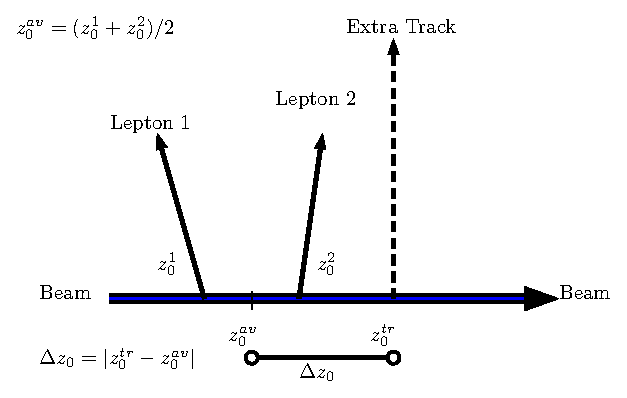
\includegraphics[width=0.8\textwidth]{figures/cartoon.eps}
\caption{Illustration of the geometry of the exclusivity selection criteria}
\label{fig:exclCartoon}
\end{figure}

\par Although \DZ\ was observed to be sensitive to pileup events, the signal selection 
efficiency in the pileup range expected during the Run I data taking period was not terrible. At 
worst the signal efficiency was about 50\%, when the number of pileup events ($\mu$) was 
greater than 30. During Run I, the average number of pileup events was 20.7. Figure~\ref{fig:pileupEff} 
shows the signal efficiency of this selection, simulated using FPMC, plotted against 
the number of pileup event, $\mu$. For $\mu=20.7$, the efficiency was found to be around 58\% 
in simulation. The was compared to the efficiency measured in data, as discussed in the 
next section. 

\begin{figure}[!h]
\centering
 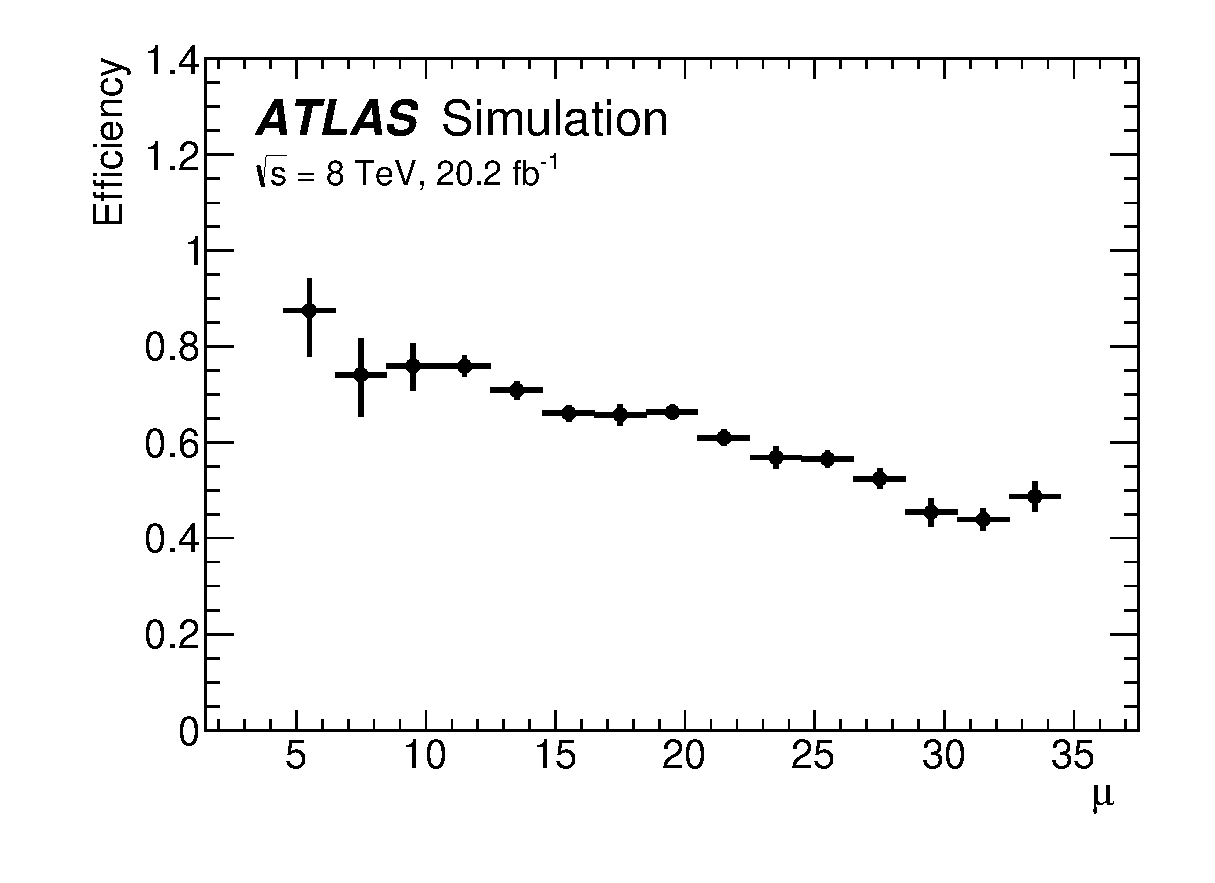
\includegraphics[width=0.8\linewidth]{figures/muFit.eps} 
\caption{Plot of the efficiency of the exclusivity selection, extracted from the
exclusive Higgs boson signal simulation, is plotted 
against the average number of interactions per beam crossing
$\mu$}
\label{fig:pileupEff}
\end{figure}

\subsection{Performance and calibration of exclusivity}
\label{sec:exclCalib}
\par The exclusivity selection introduced in the previous section was tested for several 
inconsistencies in data and simulation. First, since background rejection with this selection in 
simulation is dependent on the modelling of the underlying event, it is reasonable to 
expect difference in performance in different Monte Carlo generators as well as in data. 
Second, the equivalent photon approximation (EPA) is known to overestimate the cross section of 
elastic processes such as elastic di-leptons or elastic \Wpm\ pairs~\cite{Dyndal,Harland-Lang:2015cta}.
It was worthwhile to reproduce this over-estimation using \DZ\ as a cross check.  
Third, SD and DD Monte Carlo simulation for exclusive \Wpm\ pairs is not available. A mechanism to estimate 
these contributions was developed in the context of \DZ. 

\par This section discusses three studies. The underlying event modelling in several 
Monte Carlo generators were calibrated to match the underlying event in data. The EPA 
overestimation of elastic cross sections were reproduced using the \DZ\ selection criteria. 
SD and DD contributions to the exclusive \Wpm\ pairs was estimated. These three studies 
essentially tested the perfomance of \DZ\ and enabled its calibration.  

\subsubsection{Calibration of the underlying event}
\par To calibrate the underlying event modelling across different generators, \Zmm\ events in data 
were used for comparison. \Zee\ samples were also used separately to cross check the results. The reason for 
using Z events is that while they are a good source of leptons, they are so many in data that 
statistical uncertainties are kept at a minimum. The Z events were isolated by requiring each of the two muons 
to have at least 20~\GeV\ in \pt\ and have $80<m_{\mu\mu}<100~\GeV$. \DZ\ was then applied, essentially 
requiring no unmatched tracks in $\pm\Delta z_0<1$ mm. The $\pm\Delta z_0$ window was varied to study 
systematic uncertainties on the results. 

\par The following generators were used to simulate \Zmm\ events :
\begin{enumerate}
\item \AlpgenPythiaSix; 
\item \AlpgenHerwig;
\item \SHERPA;
\item and \POWHEG+\PYTHIAeight.
\end{enumerate} 
Figure~\ref{fig:zsubcut} shows the agreement between data and simulations from these generators. 
Circles and squares are respectively before and after the exclusivity selection was applied. Before 
exclusivity, all the generators predict \Zmm\ events to a reasonable agreement with data. After 
exclusivity, several disagreements between data and simulation, and also between simulations from the 
different generators, were observed. This is a symptom of poor underlying event modelling.  

\begin{figure}[!h]
\centering
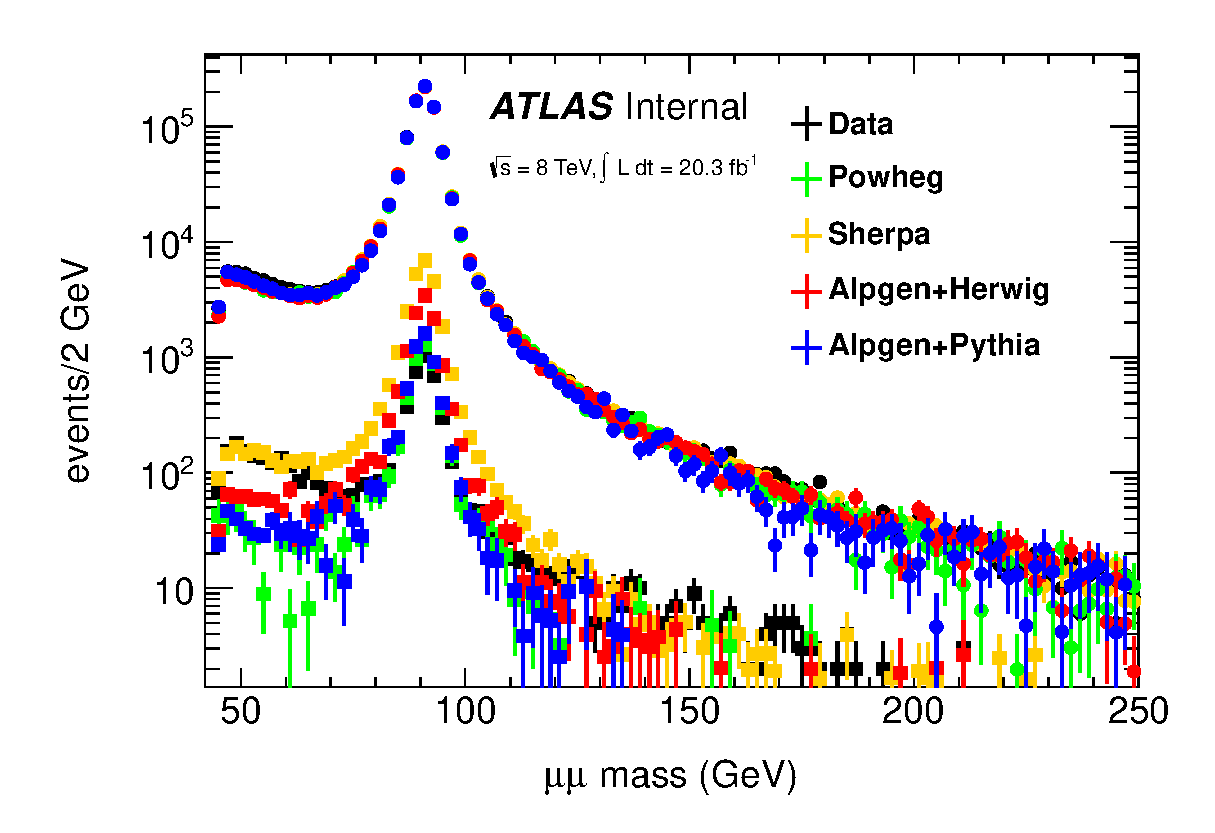
\includegraphics[width=0.8\linewidth]{figures/zrejcal.eps}
\caption{The rejection of \Zmm\ between data and simulation. Simulated samples are normalized to the
data. Circles are before \DZ\ was applied, and squares are after \DZ\ was applied}
\label{fig:zsubcut}
\end{figure}

\par The fraction of events that passed \DZ\ in simulation, $n^{exc}_{MC}/n^{inc}_{MC}$, and the fraction of events 
that passed \DZ\ in data, $n^{exc}_{data}/n^{inc}_{data}$, were compared through scale factors   

\begin{equation}
f^{sim}_{n_{trk}} = \frac{n^{exc}_{MC}/n^{inc}_{MC}}{n^{exc}_{data}/n^{inc}_{data}}, 
\label{eqn:rsf}
\end{equation}
where {\it sim} is $P$ for \POWHEG+\PYTHIAeight, $AH$ for \AlpgenHerwig, AP for \AlpgenPythiaSix,
and $S$ for \SHERPA. $n_{trk}$ is the number of tracks required in the exclusivity window, 0 
being the nominal. To improve the statistical uncertainties after \DZ, measurements with $n_{trk}$ equal 
to 1 and 1$\to$4 were also done. Exclusivity window sizes other than 1 mm were used to study 
the impact of systematic uncertainties on the results. Results for this study are shown in 
Table~\ref{tbl:rejscale}.  

\begin{table}[h]
\begin{center}
\begin{tabular}{|l|cccc|}
\hline
$n_{trk},  \Delta z^{iso}_0$ & $f^P_n$ & $f^S_n$ & $f^{AH}_n$ & $f^{AP}_n$ \\
\hline\hline
0, 1.0 mm & 0.581 & 0.128 & 0.206 & 0.692 \\
0, 1.25 mm & 0.549 & 0.113 & 0.194 & 0.679 \\
0, 1.5 mm & 0.537 & 0.103 & 0.189 & 0.663 \\
0, 2.5 mm & 0.494 & 0.084 & 0.176 & 0.613 \\
0, 4.0 mm & 0.308 & 0.074 & 0.170 & 0.579\\
1-4, 1.0 mm & 0.876 & 0.571 & 0.393 & 0.853 \\
1, 1.5 mm & 0.681 & 0.324 & 0.247 & 0.736 \\
\hline
\end{tabular}
\caption{Measured $f^{sim}_{n_{trk}}$ values for several different Monte Carlo generators, under different exclusivity 
settings. Exclusivity window sizes other than 1 mm were used to study the impact of systematic variations on the results.} 
\label{tbl:rejscale}
\end{center}
\end{table}

\par To use the scale factors in Table~\ref{tbl:rejscale} to calibrate processes other than $Z$ decays 
these scale factors were extrapolated to a wider di-muon mass range. In particular, the stability of event
yields after imposing \DZ\ at di-muon masses other than between 80 and 100~\GeV needed to be quantified. These simulation yields 
 were measured in bins of $44\to60~\GeV$, $60\to90~\GeV$, $90\to116~\GeV$ and $116\to200~\GeV$. In all bins, \SHERPA had the 
minimal statistical uncertainties, so its results were compared to those from the other three generators. Quantities 
shown in Table~\ref{tab:gencm} are ratios of yields from the different generators to the yields from \SHERPA after 
the \DZ\ selection. A generous 20\% variation on the nominal yield (\SHERPA) covers yields from all other 
generators.  

\begin{table}
\begin{center}                                                                 
\begin{tabular}{l|c|c|c}                                                       
\hline                                                    
Mass [\GeV]  & \AlpgenHerwig & \AlpgenPythiaSix  & \PowhegPythiaEight  \\    
\hline         
 44--60  & $0.81 \pm 0.02$  & $0.84 \pm 0.03$ & $0.99 \pm 0.09$\\     
 60--90 & $1.04 \pm 0.02$  & $0.98 \pm 0.03$  & $1.01 \pm 0.02$\\     
 90--116 & $1.00 \pm 0.01$ & $1.02 \pm 0.02$  & $1.00 \pm 0.02$ \\  
 116--200 & $0.89 \pm 0.10$& $1.04 \pm 0.19$  & $0.76 \pm 0.10$\\    
\hline      
\end{tabular}                     
\caption{Ratio of the exclusivity selection efficiency in Drell-Yan
 $\mu^+\mu^-$
production as a function of dimuon mass of different generators to
\SHERPA. Only statistical uncertainties 
are shown. The statistical uncertainty from \SHERPA is included and contributes $2.9\%, 0.8\%,
0.7\%$ and $5.7\%$ in the four mass regions.}
\label{tab:gencm}            
\end{center}             
\end{table}

%\par Talk about validation of scale factors ... show Figure 7 from the paper ...


\subsubsection{Di-lepton check}
\label{sec:acofit}
\par As mentioned above, the EPA is known to overestimate the elastic contribution to exclusive processes 
that occur by exchanging a pair of photons. This section discusses a study that reproduces this overestimation 
within uncertainties, thereby validating \DZ. 

\par Since elastic, SD and DD Monte Carlo simulation samples for exclusive di-leptons were available, exclusive 
di-leptons were used for this study. The strategy was to isolate exclusive di-muons in data, entangle the 
elastic component, and compare it with the prediction from EPA. From this comparison, a scale factor than normalizes 
the EPA prediction to data was extracted and compared to previous studies of a similar nature. The basic selection required 
that each of the muons have $\pt>20~\GeV$, $m_{\mu\mu}>45~\GeV$ excluding a $\pm15~\GeV$ window around the 
\Zboson\ mass, and \DZ. Elastic di-muons tend to populate the low \pTmumu\ region, as shown in 
Figure~\ref{fig:ptL}, where all the basic selection criteria described above were applied. 
So, a selection of $\pTmumu<3~\GeV$ was additionally applied.  
The major background 
to the exclusive di-muons in this region was Drell-Yan di-muons; every other background was negligible.  
Clearly, in Figure~\ref{fig:ptL} there is an overestimation of processes from simulation. 

\begin{figure}
\centering
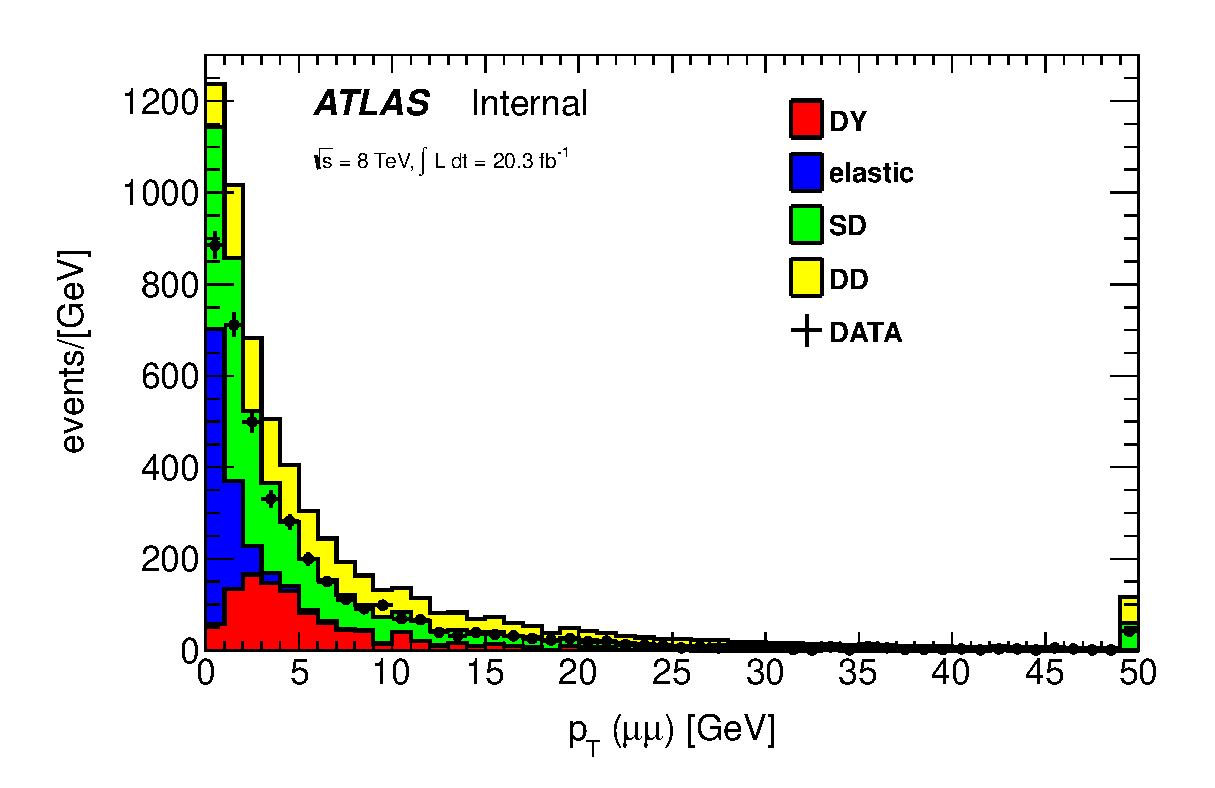
\includegraphics[width=0.8\linewidth]{figures/ptmumuL.eps}
\caption{Plots showing the exclusive (1.0 mm) di-muon $p_{\mathrm{T}}^{\mu\mu}$ distributions predicted and observed. The
  highest bin includes overflow. No scale factors are applied to
  elastic or SD or DD predictions}
\label{fig:ptL}
\end{figure}

\par Acoplanarity, defined as $1-\Delta\phi_{\mu\mu}/\pi$, is a good discriminant when disentangling elastic 
from SD and DD processes. This is expected, since $\Delta\phi_{\mu\mu}$ is dependent on \pTmumu. In this study, 
acoplanarity distributions from simulation after applying the selection criteria described in the preceding paragraphs   
were fit to the acoplanarity distribution from data, after the same selection criteria was applied. 
The yields from the fit were then extracted, comparing the elastic prediction to data minus everything else. 

\par The acoplanarity distributions before the fit are shown in Figure~\ref{fig:shapes}. Clearly, SD, DD and 
Drell-Yan have similar shapes. For the fit, SD, DD and Drell-Yan contributions were summed up and treated as 
one process. The Drell-Yan background was varied by $\pm20\%$ to evaluate systematic variations in modelling 
$f^{sim}_{n_{trk}}$. The binning and range of acoplanarity distributions were also varied to evaluate 
systematic uncertainties. These uncertainties were shown to impact results by about 7\%. 
Figure~\ref{fig:dilepAcoFit3Shape} shows the post-fit acoplanarity distributions, with 
simulation stacked on top of each other and the total agreeing with the data. From this fit a scale factor 
 $f_{EL}$ = 0.76 $\pm0.04$ (stat.) $\pm0.07$ (sys.) was extracted. This value agrees within uncertainties with 
previous predictions~\cite{Dyndal}, which cover a range between 0.73 and 0.75.   

\begin{figure}[!h]                                                                 
\centering
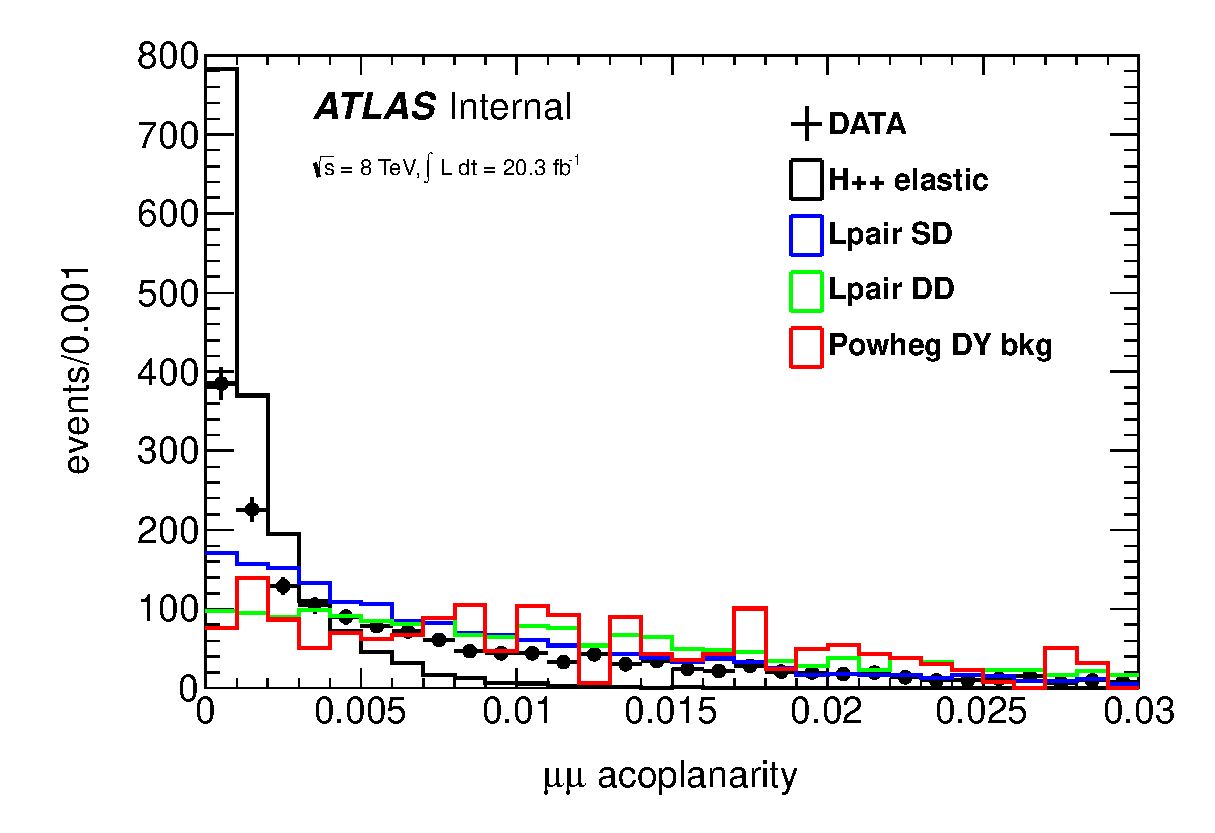
\includegraphics[width=0.8\linewidth]{figures/shapes.eps}     
\caption{Plots of acoplanarity distributions for elastic, SD, DD and Drell-Yan
each normalized to the data}                                             
\label{fig:shapes}                        
\end{figure} % 

\begin{figure}[!h]                                                                 
\centering
 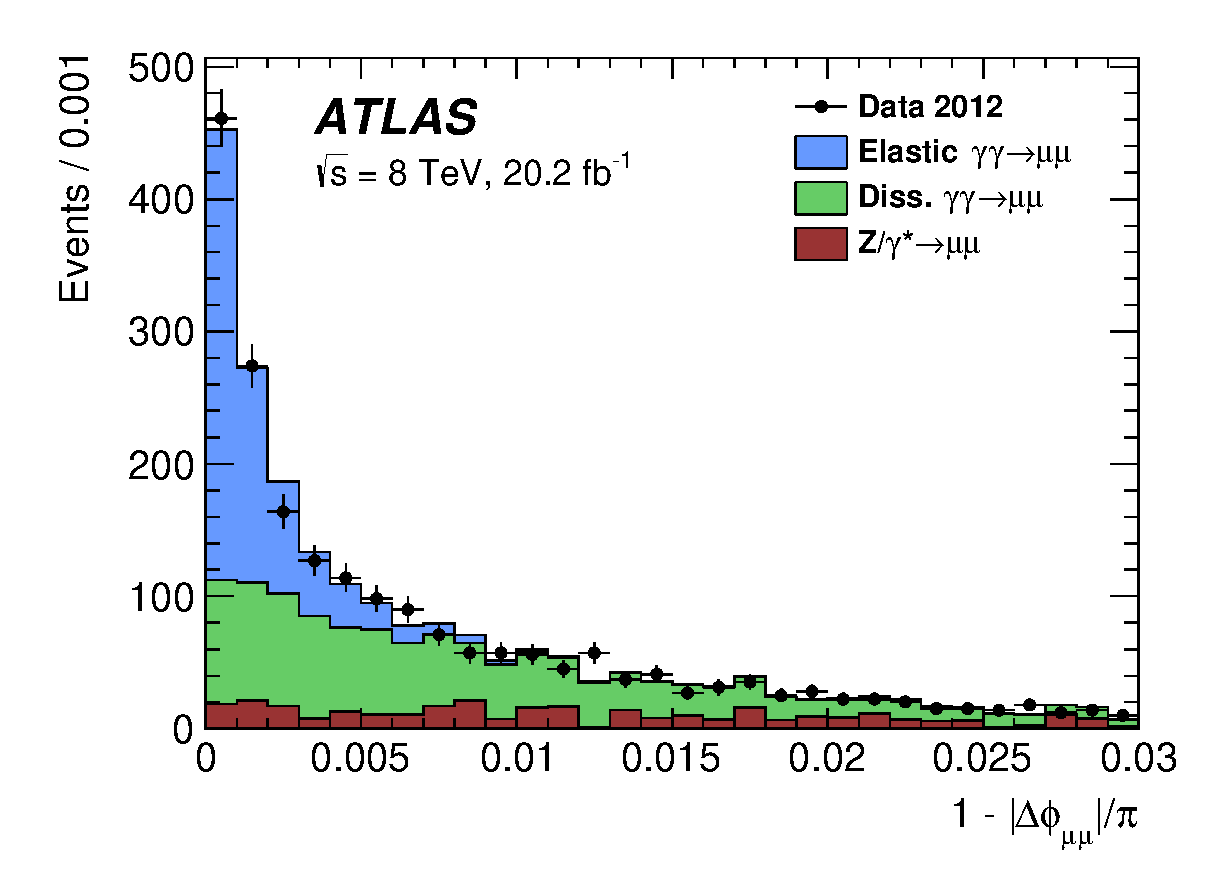
\includegraphics[width=0.8\linewidth]{figures/dilepton_3shapes_Washington_filled.eps} 
 \caption{Plots of dimuon acoplanarity distributions after applying the
 exclusivity selection and requiring $\pT^{\mu\mu} < 3$~\GeV. The 
 expected Drell-Yan shape and the 
 elastic and combined SD and DD (Dissociative) shapes normalized from
 the fit are stacked. This fit 
          determines the factor $\fEL$.}
 \label{fig:dilepAcoFit3Shape}
\end{figure}                                        

\par A separate study independent of the fit method was also done to test the robustness of \fEL. 
This involved making an explicit selection based on acoplanarity in addition to the basic requirements 
already discussed above, counting the yields and re-calculating an estimate to \fEL. For acoplanarity less than 0.003, 
899 events were observed in data, 764 elastic dimuons were predicted by EPA, and 340, 67 and 64 SD, DD and Drell-Yan 
events were also predicted respectively. This corresponds to an estimate to \fEL\ of 
 $0.71 \pm0.03 \text{(stat)} \pm0.01 \text{(sys)}$. 
Similarly, tightening the acoplanarity selection to be less than 0.0015 yielded 0.73 $\pm0.03 \text{(stat)} \pm0.01 \text{(sys)}$.
These results fall well within the uncertainties of the results obtained from the fit method. 

\par \DZ\ was tested for robustness against pileup by testing its performance in events with a selection identical to 
the one prior to the fit plus an acoplanarity cut, with the difference that one extra track was allowed in the exclusivity 
window. For exclusive processes, this extra track has to be from pileup because there is no underlying 
event. As such, the $\Delta z_0$ between this extra track and the di-lepton vertex is expected to be 
uniformly distributed, showing no clear peaks. Figure~\ref{fig:dzEventOneTrk} shows the  $\Delta z_0$ 
distributions for the extra track in exclusive and \Zmm\ events. For exclusive processes these 
distributions are uniform while for \Zmm\ a they peak at 0. This shows that for \Zmm\ the extra track 
is from the underlying event. The acoplanarity cut was tightened and loosened and an estimate of \fEL\ was 
computed at each variation. All the \fEL\ estimates fell within $\pm10\%$, showing that \DZ\ has an a 10\% 
pileup uncertainty.   

\begin{figure}[!h]
\centering
 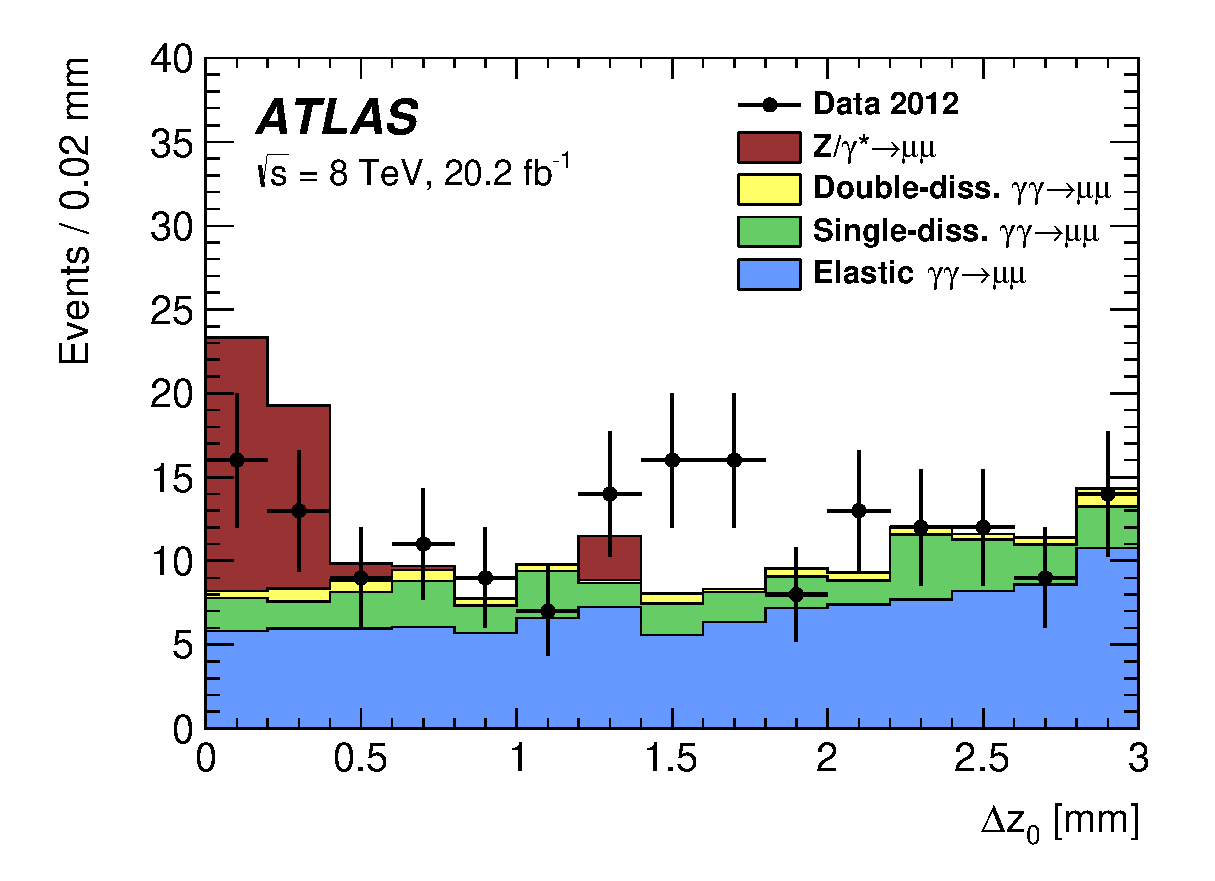
\includegraphics[width=0.8\linewidth]{figures/dilepton_dzone15.eps} 
 \caption{Plots of absolute $\Delta z_0$ of the extra track to the lepton vertex 
          in the region defined by acoplanarity $<0.0015$. The exclusivity 
          requirement was changed to select exactly one
          extra track within 3~mm.  The exclusive predictions are
 scaled by a factor of 0.70}
 \label{fig:dzEventOneTrk}
\end{figure}

\par Since electrons are also in the signal final state, these studies were repeated using 
\Zee\ events. Due to the fact that electrons undergo brehmsstrahlung at a much higher rate than 
muons, results in the \Zee\ channel carried a much higher error. In particular, when an electron 
radiates a photon (which pair produces electrons), the extra track that the radiated electron produces 
in the ID may be counted as an extra track by \DZ. This phenomenon is referred to here as 
{\it electron self-veto}. For acoplanarity less than 0.003 the estimate to \fEL\ obtained 
through \Zee\ events was about 0.67. For acoplanarity less than 0.0015 it was 0.68. These results 
correspond to a $3.0\pm 2.5\%$ difference with the results obtained from \Zmm. This difference was 
taken as the uncertainty due to the electron self-vetoing itself.   

\subsubsection{Photon flux}
\label{sec:flux}
\par This section discusses the estimation of SD and DD \Wpm\ contributions to the exclusive 
\Wpm\ pair production. This is an important estimation because it propagates to the estimation of 
the exclusive \Wpm\ pair contamination in the exclusive Higgs boson signal region.  

\par Since exclusive di-lepton production is identical to exclusive $\WW$ production, 
this study was conducted with exclusive di-leptons. The results were then 
applied to exclusive $\WW$. The strategy was to isolate exclusive di-leptons with high mass  
in data and taking the ratio of the data minus background to the elastic di-lepton prediction. 
This ratio was then applied to the elastic $\WW$ prediction to account for the SD and DD contributions. 
As before the leptons used were di-muons, each of at least 20~\GeV\ in \pt. To suppress di-muons from 
$\WW$ decays, $m_{\mu\mu}$ was required to be at least 160~\GeV. After applying \DZ, 244 events were 
observed in data were 17.4 was predicted to be from Drell-Yan, 0.4 from inclusive $\WW$ and 2.4 from exclusive 
$\WW$. The predictions were corrected using the $f^{sim}_{n_{trk}}$ calibrations. From these quantities a scale factor 

\begin{equation}
 \fgam = \frac{N_{\mathrm{Data}} 
              - N^{\POWHEG}_{\mathrm{Background}}}{N^{\HERWIGPP}_{\mathrm{Elastic}}} \Bigg\rvert_{m_{\mu\mu} > 160~\GeV}
            = 3.30 \pm 0.22 \mathrm{(stat.)} \pm 0.06 \mathrm{(sys.)},
 \label{eqn:fgamma}
\end{equation}
was calculated, where $N_{\mathrm{Data}}$ is the number of events in data, 
$N_{\mathrm{Background}}^{\POWHEG}$ is the expected number of
background events, 
and $N_{\mathrm{Elastic}}^{\HERWIGPP}$ is the expected number of elastic $\yymumu$ candidates
directly from \HERWIGPP, i.e, the unscaled EPA prediction. 
Drell-Yan processes were the major contribution to the total background events and inclusive 
and exclusive $\WW$ contributed less than 10\%. To estimate the systematic uncertainties, the Drell-Yan 
contribution was varied by $\pm20\%$. Figure~\ref{fig:fluxM160} shows the $m_{\mu\mu}$ and 
$m_{ee}$ distributions for the exclusive di-leptons after applying \fEL\ to the elastic contribution 
and scaling the SD distribution such that the sum of the elastic and SD contributions corresponds 
to $\fgam \times N_{\mathrm{Elastic}}^{\HERWIGPP}$. These corrected predictions agree very well with the data. 

\begin{figure}
 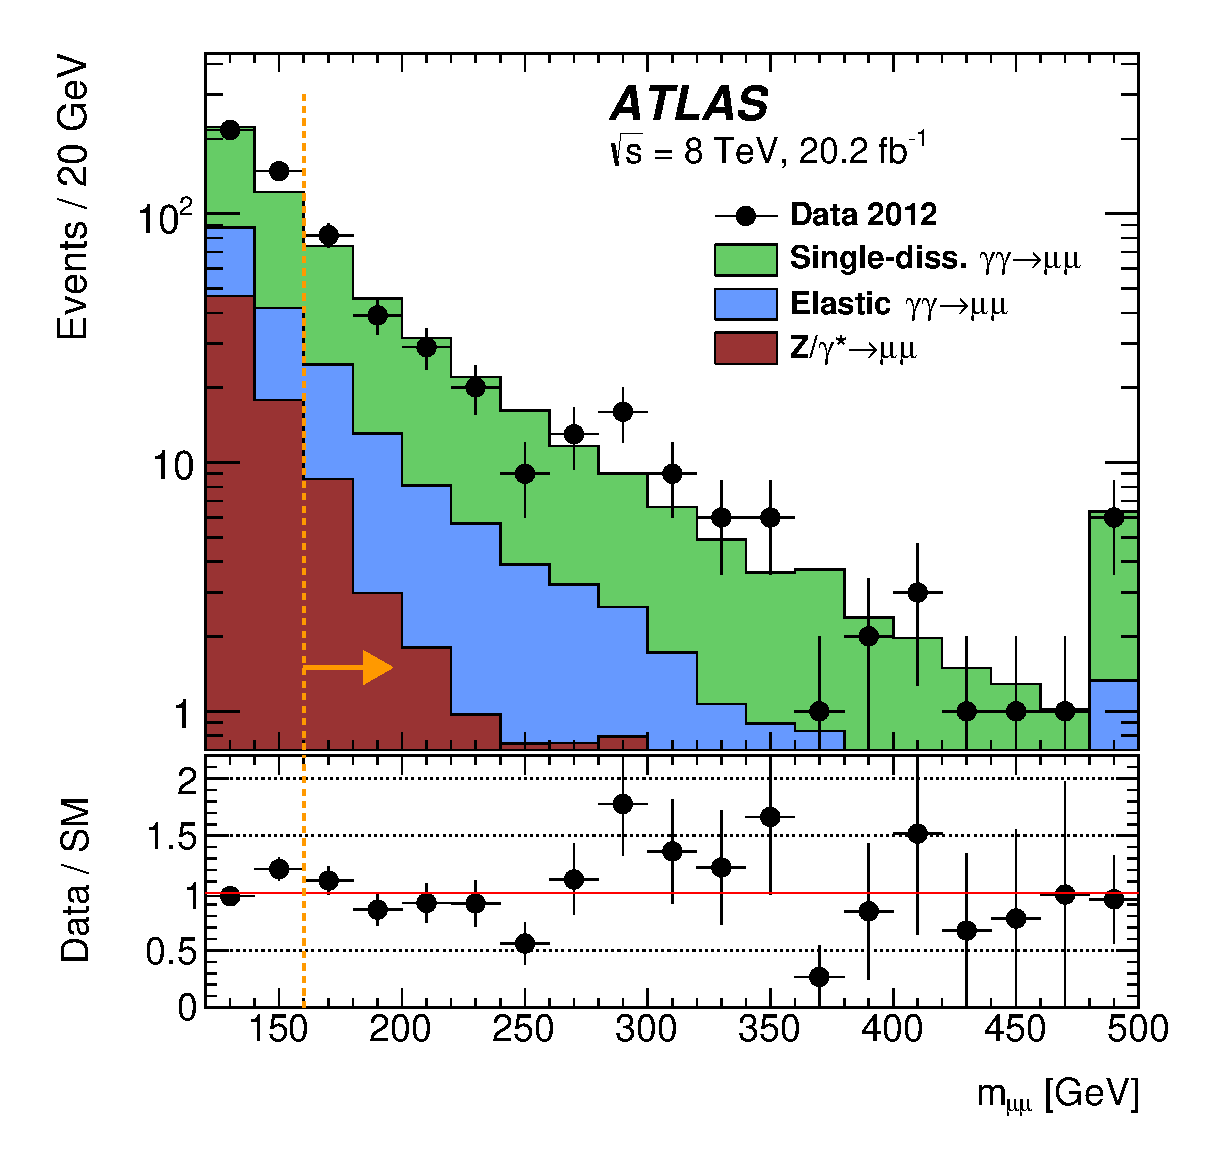
\includegraphics[width=0.5\linewidth]{figures/flux_m160mumu.eps} 
 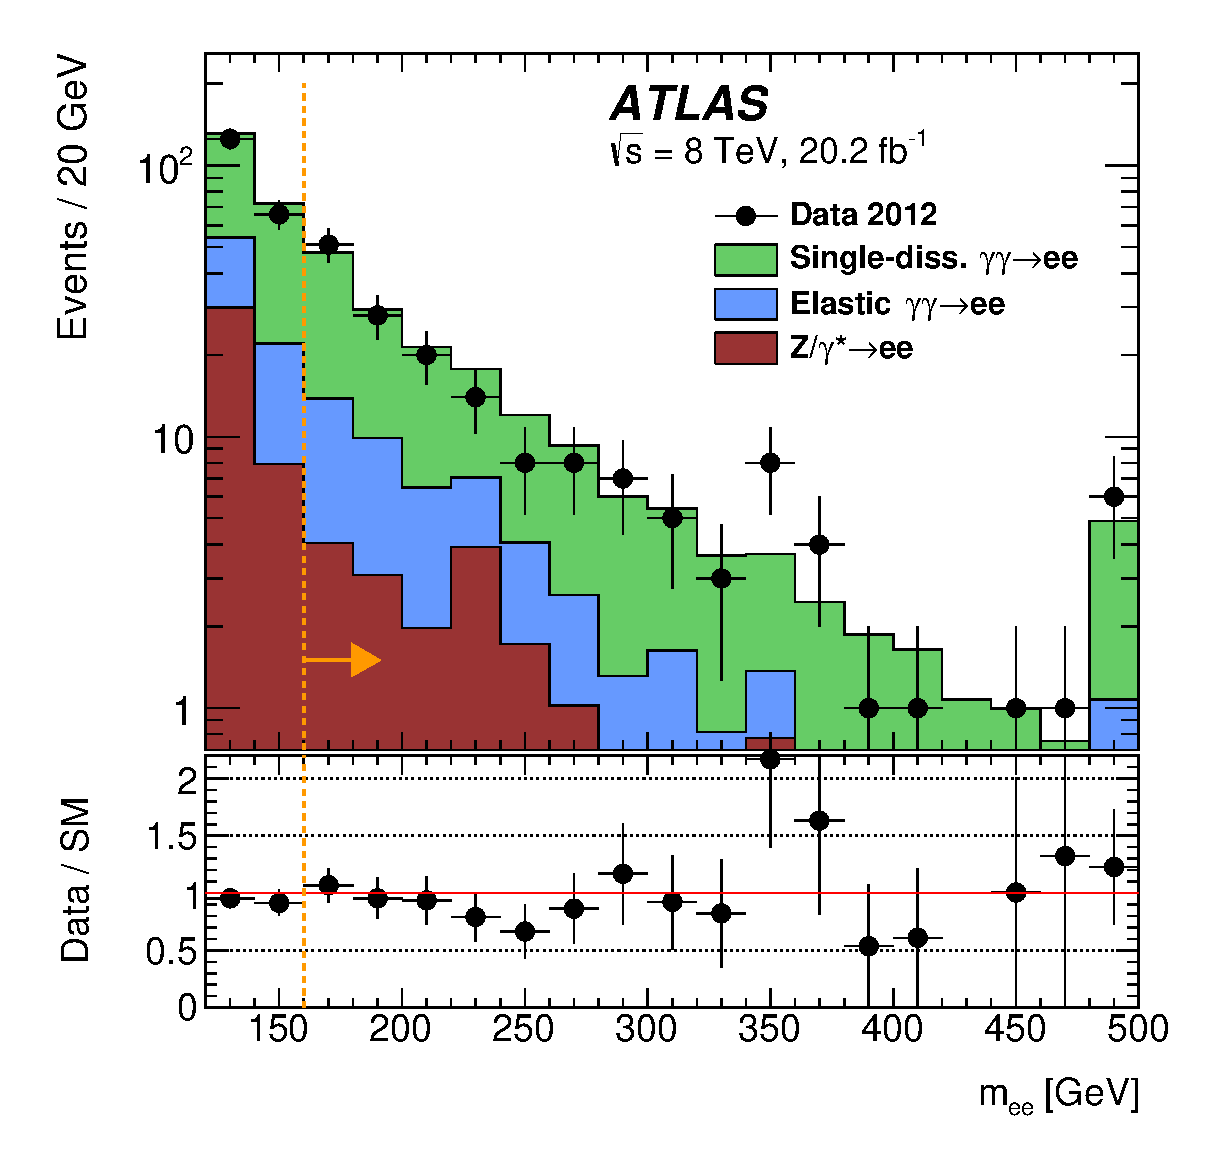
\includegraphics[width=0.5\linewidth]{figures/flux_m160ee.eps} 
 \caption{Plots of the dilepton invariant mass distribution for muon
 candidates (left) and 
          electron candidates (right). The elastic yield is scaled 
          by $\fEL = 0.76$ and the SD distribution is scaled to
          bring the sum of the elastic and SD contributions to the 
          \HERWIGPP prediction for the elastic process multiplied by
          the $\fgam$ factor in the mass region above
          160~\GeV. The last bin includes overflow}
 \label{fig:fluxM160}
\end{figure}

\par The distributions in Figure~\ref{fig:fluxM160} show that while \fgam\ was extracted from the 
invariant di-lepton mass greater than 160~\GeV, its value is rather insensitive to this choice of 
cut.

\par From the above-mentioned di-muon sample in data, the \DZ\ selection efficiency was measured. It was 
observed to be $0.58\pm0.06$, where the 10\% uncertainty arose from pileup modelling. This measurement 
agrees very well with the \DZ\ efficiency measured 
in the exclusive Higgs boson signal samples.      



\section{Modelling of background processes}
\label{sec:bkgExclH}
\par Backgrounds to the signal region, as defined in Section~\ref{sec:selExclH}, are categorized 
into exclusive and inclusive backgrounds. This section discusses modelling of these backgrounds in 
light of the scale factors that have been discussed so far.  

\subsection{Exclusive backgrounds}
Figure~\ref{fig:prelimMT} shows that the only major exclusive 
background expected to contaminate the signal region exclusive \WW, even though several selection criteria listed in 
Table~\ref{tab:evSel} were dedicated to suppressing the \WW\ spectrum. As discussed in Section~\ref{sec:exclCalib}, 
SD and DD simulation samples for exclusive \WW\ do not exist. \fgam, defined in Equation~\ref{eqn:fgamma}, 
was applied on the \HERWIGPP\ prediction of elastic \WW\ to account for the SD and DD components of exclusive \WW. 
No other corrections were applied. Section~\ref{sec:exclWWCR} discusses a dedicated region in data used to  
validate modelling of exclusive \WW.    

\par The second significant exclusive background to the signal region is exclusive di-leptons, specifically 
exclusive \yytautau. The different flavor selection criteria suppresses all the other exclusive di-leptons 
to the extent that they are insignificant. \fgam\ was also applied on the \HERWIGPP\ prediction of elastic 
\yytautau\ to account for the SD and DD contributions to the exclusive \yytautau. Since exclusive di-leptons 
are produced in a manner similar to exclusive \WW, the exclusive \WW\ validation 
region in data hinted in the preceding paragraph also serves to validate modelling of exclusive di-leptons.

\par No other exclusive backgrounds significantly contaminated the signal region.    

\subsection{Inclusive backgrounds}
\par Figure~\ref{fig:prelimMT} shows that the major inclusive backgrounds that contaminate the signal region are 
inclusive \WW, $VV$, $V$+jets and Top. $VV$ backgrounds are a collection of all non-\WW\ processes such as 
$ZZ$, $ZW$ and $W\gamma$. $V$+jets are a collection of $W$+jets and Drell-Yan. Top backgrounds are the sum of \ttbar\ and 
single-top processes. Figure~\ref{fig:prelimMT} also shows that the most dominant of all of these 
inclusive processes was inclusive \WW. Estimation of inclusive \WW's estimation was rather complex. 
Several calibrations and corrections were made on the original \PYTHIAeight\ prediction. These calibrations 
and corrections are discussed in the next two sub-sections. 

\par From Figure~\ref{fig:prelimMT} it is clear that while inclusive \WW\ events were expected to dominate 
inclusive backgrounds, the sum of all other inclusive backgrounds was expected to be significantly less than the 
inclusive \WW\ contribution. For this reason, all inclusive backgrounds, apart from inclusive \WW, were sometimes 
treated collectively. The next sub-sections clarify this strategy.   

\subsubsection{Inclusive \WW\ normalization}
\par From previous measurements~\cite{ATLAS:2014aga,Aad:2016wpd}, it is known that the NLO prediction for the $q\bar{q}\rightarrow W^{+}W^{-}$
 process as provided by \PowhegPythiaEight\ underestimates the observed inclusive $\WW$ event yield. 
It was therefore necessary to understand the simulation of this background before requiring the exclusivity selection. 
A control region close in phase space to the signal region was chosen for this purpose.
 It had the same definition as the signal region except: $55 < \memu < 110~\GeV$,  
$\dFem<2.6$ to reduce Drell-Yan background, no jets to reduce \ttbar\ background, and no requirement on exclusivity.
This region was dominated by inclusive $\WW$ production, with a purity of 60\%. 

\par After subtracting the predicted backgrounds 
from data, $(20 \pm 5)\%$ more data was observed than is predicted
by \PowhegPythiaEight. To correct for this, a normalization factor of $1.20 \pm 0.05$(stat.)
was therefore taken as a correction to the cross-section and applied to the inclusive $\WW$ prediction in all regions 
of phase space, as done in Ref.~\cite{ATLAS:2014aga}. A summary of the event yields in this region, where the 
inclusive \WW\ prediction was scaled by $1.20 \pm 0.05$(stat.), is shown in Table~\ref{tab:WWyields}.  
Several kinematic distributions in this control region
after applying the normalization factor to the \PowhegPythiaEight\ prediction are also 
shown in Fig.~\ref{fig:incWWplots}. Clearly, the Monte Carlo predictions agree reasonably 
well with data observations. 

\begin{table}
\centering
\begin{tabular}{|l|c|}
\hline
		Background                 & Event Yield \\
\hline\hline
    Inclusive $\WW$             & 1913.54 $\pm$ 8.78 \\
    $VV$               					& 369.65 $\pm$ 195.60  \\
    \ttbar           					  & 211.39 $\pm$ 1.79 \\
		$W$+jets										& 196.47   $\pm$ 24.40 \\
		\Ztau												& 160.08 $\pm$ 4.91 \\
		Single Top                  & 112.09 $\pm$ 1.37 \\
		Other 											& 36.39  $\pm$ 0.25 \\	
    \hline
    Total SM                    & 2999.61 $\pm$ 197.42  \\
    Data                        & 2995             \\
\hline
\end{tabular}
\caption{Summary of background yields in the control region used to correct \PowhegPythiaEight's 
prediction of inclusive \WW\ processes.}
\label{tab:WWyields}
\end{table}

\begin{figure}[!h]
\begin{subfigure}{0.5\textwidth}
   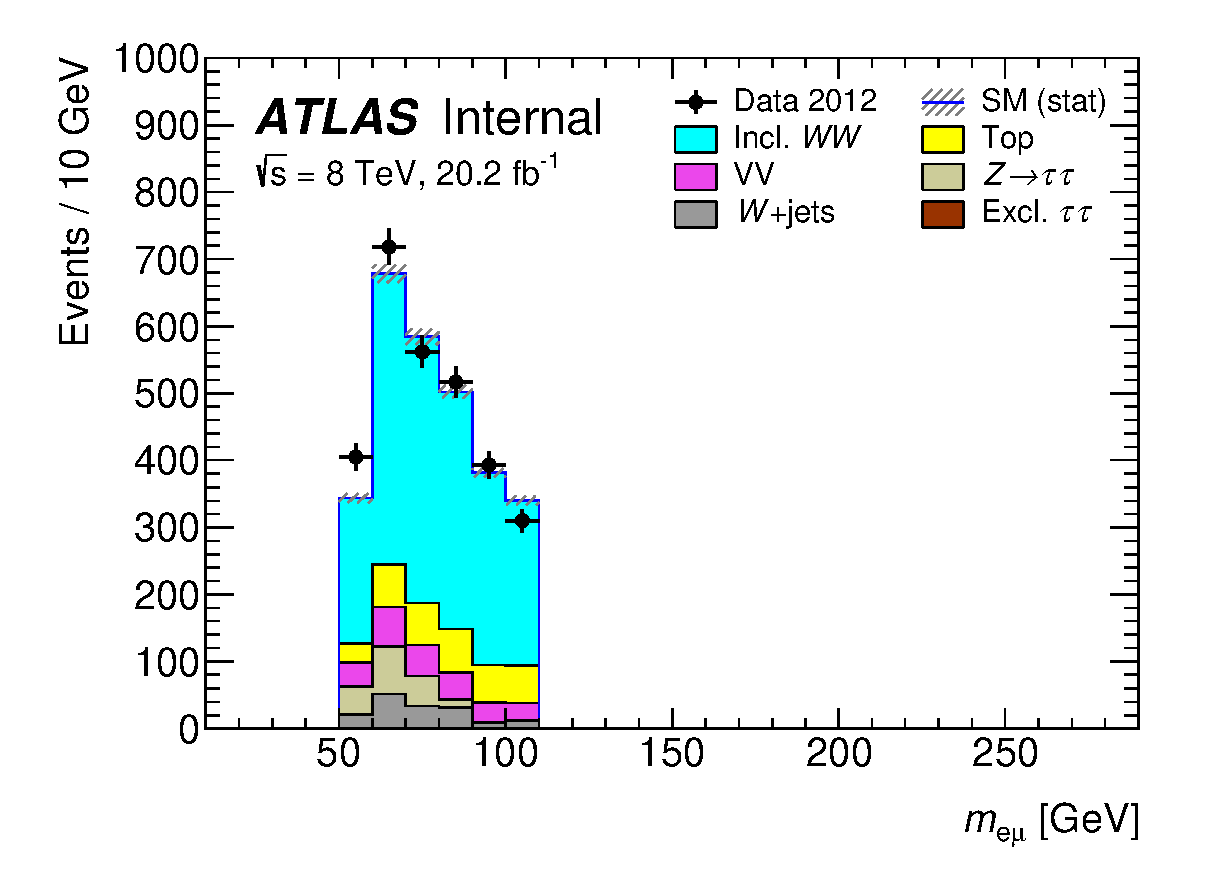
\includegraphics[width=\textwidth]{figures/emme-CutNjets-Mll-lin.eps}
\end{subfigure}
\begin{subfigure}{0.5\textwidth}
   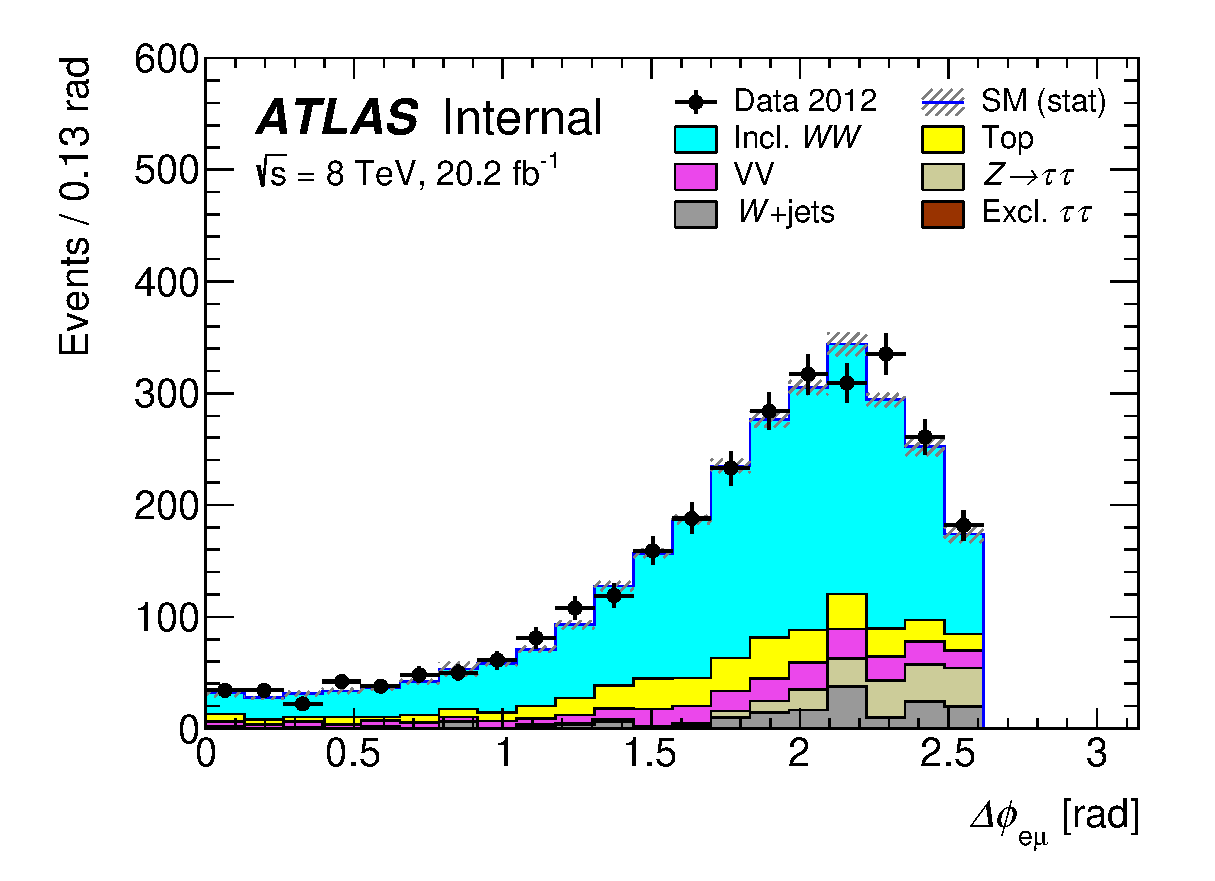
\includegraphics[width=\textwidth]{figures/emme-CutNjets-DPhill-lin.eps}
\end{subfigure} 
\begin{subfigure}{0.5\textwidth}
   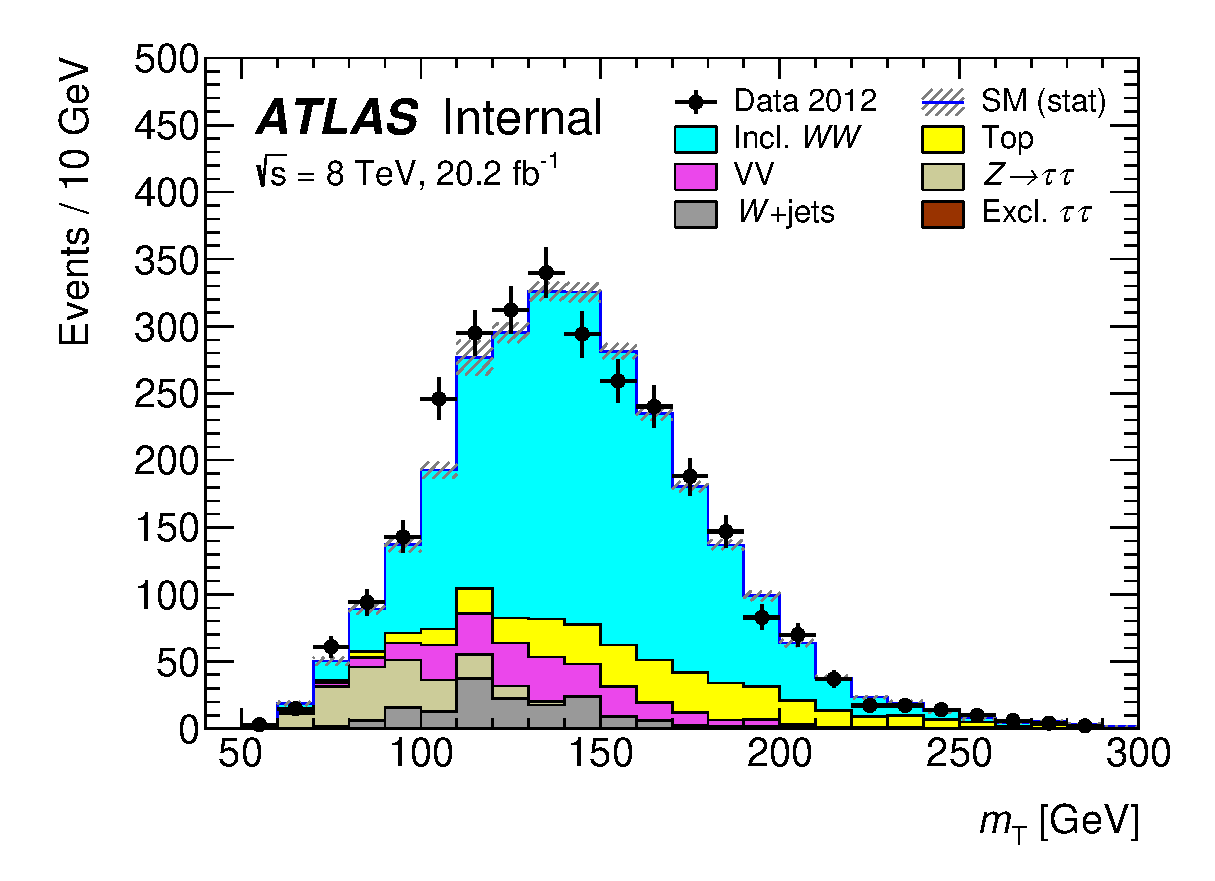
\includegraphics[width=\textwidth]{figures/emme-CutNjets-MT-lin.eps}
\end{subfigure} 
\begin{subfigure}{0.5\textwidth}
   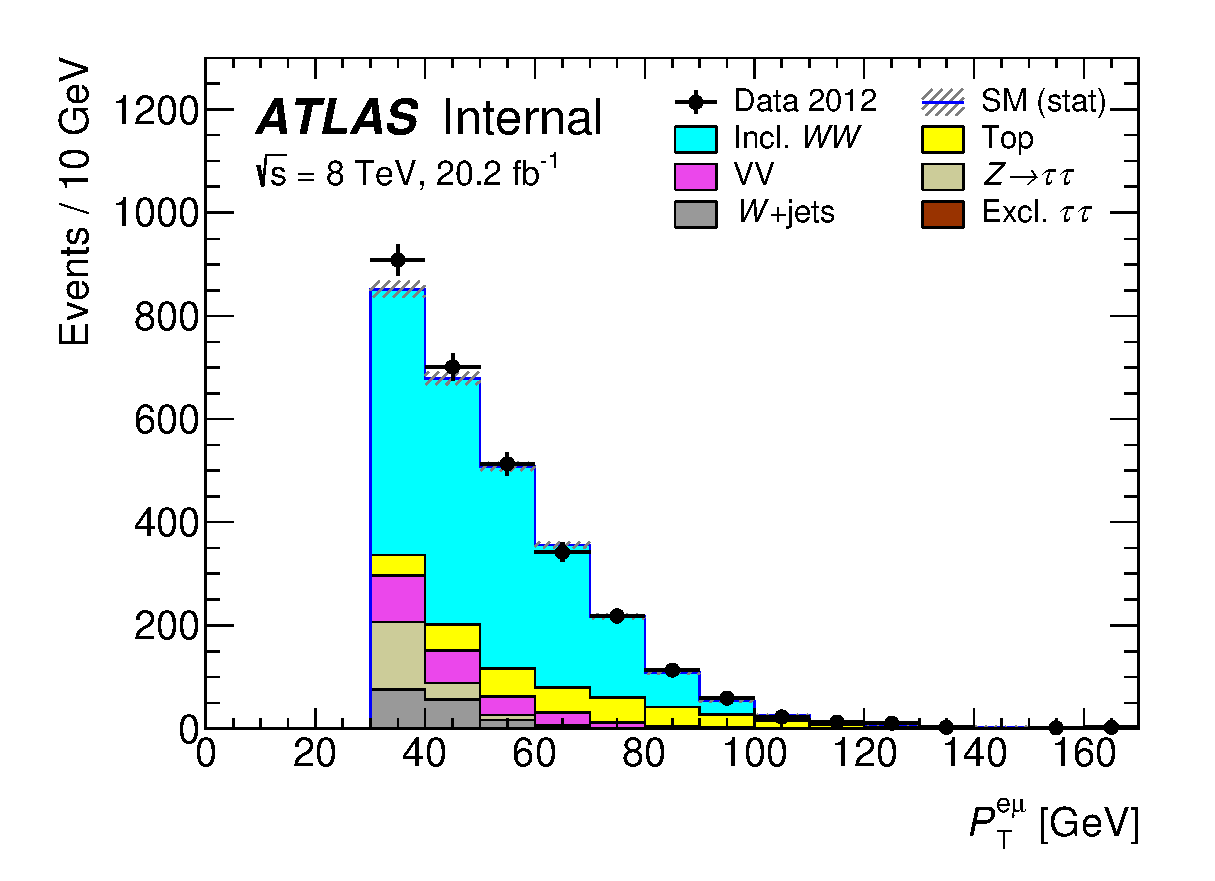
\includegraphics[width=\textwidth]{figures/emme-CutNjets-Ptll-lin.eps}
\end{subfigure} 
\caption{Plots showing \memu, \dFem, \mT\ and \pTemu\ distributions in an inclusive $\WW$-rich region}
\label{fig:incWWplots}
\end{figure}


\subsubsection{Inclusive \WW\ and other backgrounds}
\label{sec:incWW}
\par While the study discussed in the preceding sub-section demonstrates that the inclusive 
\WW\ prediction after correction with the $1.20 \pm 0.05$(stat.) normalization factor was reasonable, 
validation of modelling of inclusive \WW\ after the exclusivity selection was necessary. 
A dedicated control region in data that isolated inclusive \WW\ events to a reasonable 
purity was defined for this purpose. The region definition is listed in Table~\ref{tab:incWWCR}. 

\begin{table}
\centering
\begin{tabular}{|l|c|}
\hline
                                & Selection \\
\hline\hline
& \\
\multirow{3}{*}{Preselection } & Oppositely charged $e\mu$ final states   \\
                                				&  $\pT^{\ell 1} > 25~\GeV$ and $\pT^{\ell 2} > 20~\GeV$ \\
																		    & $\memu > 20~\GeV$     \\
& \\
\hline
& \\
				& $\pTemu > 30~\GeV$\\
                          & Exclusivity selection, allowing 1 to 4 tracks\footnote{\DZ\ allows 0 tracks in 
the exclusivity window.}\\
& \\
\hline
\end{tabular}
\caption{Selection criteria for the region used to study inclusive \WW\ events.}  
\label{tab:incWWCR}
\end{table}

\par The strategy here was to loosen the exclusivity selection slightly by allowing 1 to 4 extra 
tracks in the exclusivity window rather than allowing 0 tracks. While this loose selection allowed 
many inclusive \WW\ events to be selected, rejection of other backgrounds  
was rather unoptimized. These backgrounds are $W$+jets, Drell-Yan and Top. They are referred to here 
as {\it Other Backgrounds}. Exclusive processes such as exclusive \WW\ and exclusive \yytautau, being well 
calibrated by \fgam, were subtracted from the data. This strategy therefore studies the sum of   
inclusive \WW\ and other backgrounds. Expected and observed event yields in this data 
region are listed in Table~\ref{tab:xtrkWWEventYields}, and kinematic distributions are 
shown in Figure~\ref{fig:xtrkWWplots}. 

\begin{table}[!h]
   \centering
   \begin{tabular}{l|c}
     \hline\hline
    Processes & Inclusive $\WW$ \\
    \hline\hline
    Inclusive $\WW$             & 102 $\pm$ 20 \\
    Exclusive $\WW$             & 5.5 $\pm$ 0.4 \\
    Exclusive $\tau^+\tau^-$    & 1.2 $\pm$ 0.2 \\
    Other diboson               & 10.9 $\pm$ 2.2  \\
    Other background            & 27.4 $\pm$ 6.2 \\
    \hline
    Total SM                    & 147 $\pm$ 21  \\
    Data                        & 191             \\
    \hline\hline                                  
   \end{tabular}
  \caption{Event yields in the inclusive $\WW$-rich region.}
  \label{tab:xtrkWWEventYields}
\end{table}

\begin{figure}[!h]
\begin{subfigure}{0.5\textwidth}
   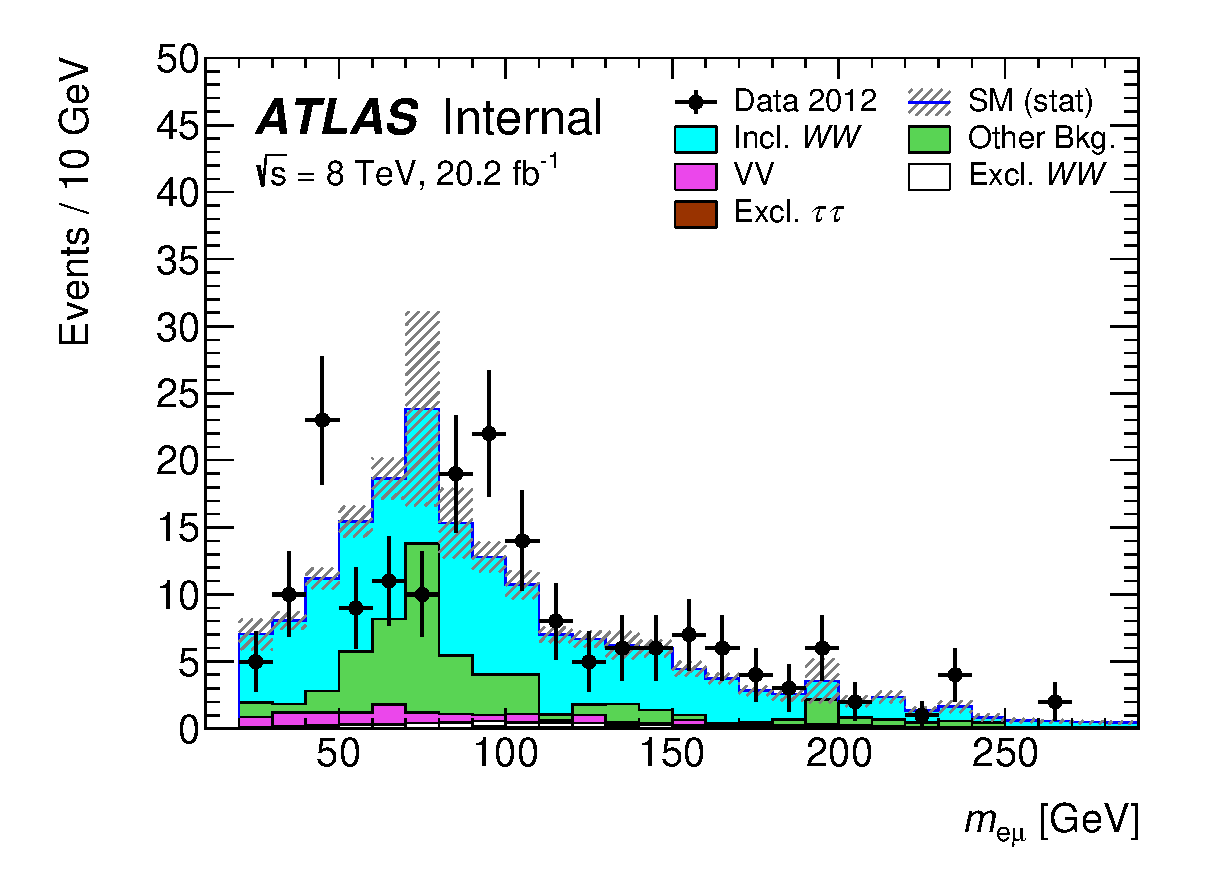
\includegraphics[width=\textwidth]{figures/emme-xtraTracks-Mll-lin.eps}
\end{subfigure}
\begin{subfigure}{0.5\textwidth}
   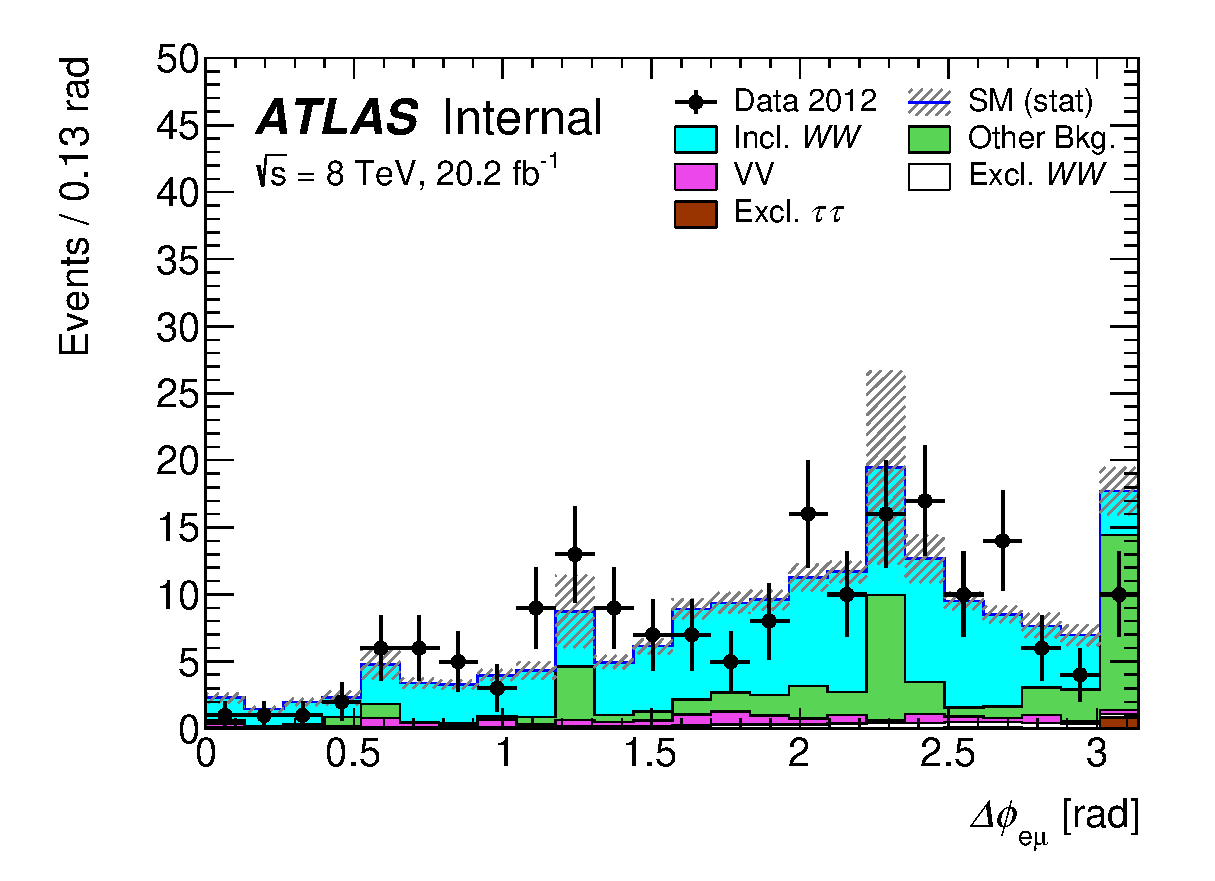
\includegraphics[width=\textwidth]{figures/emme-xtraTracks-DPhill-lin.eps}
\end{subfigure} 
\begin{subfigure}{0.5\textwidth}
   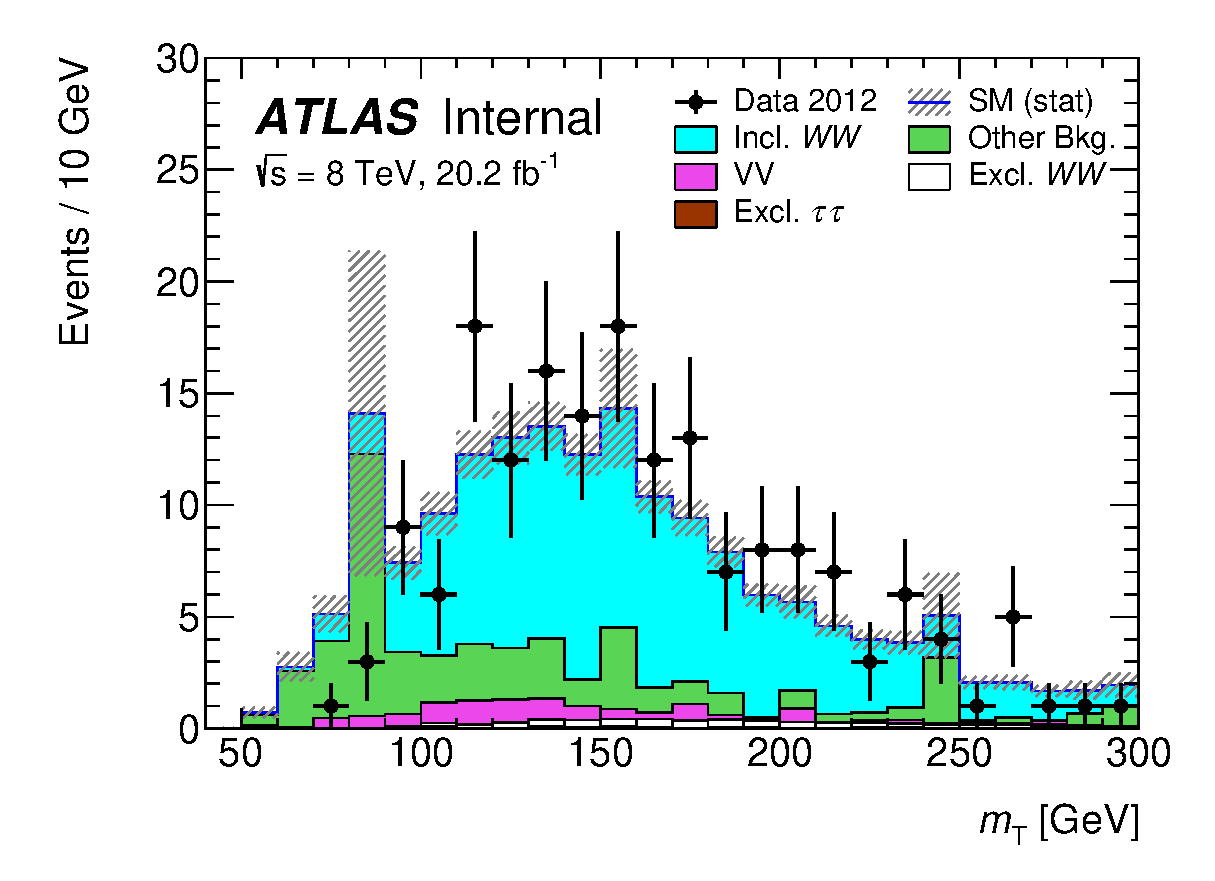
\includegraphics[width=\textwidth]{figures/emme-xtraTracks-MT-lin.eps}
\end{subfigure} 
\begin{subfigure}{0.5\textwidth}
   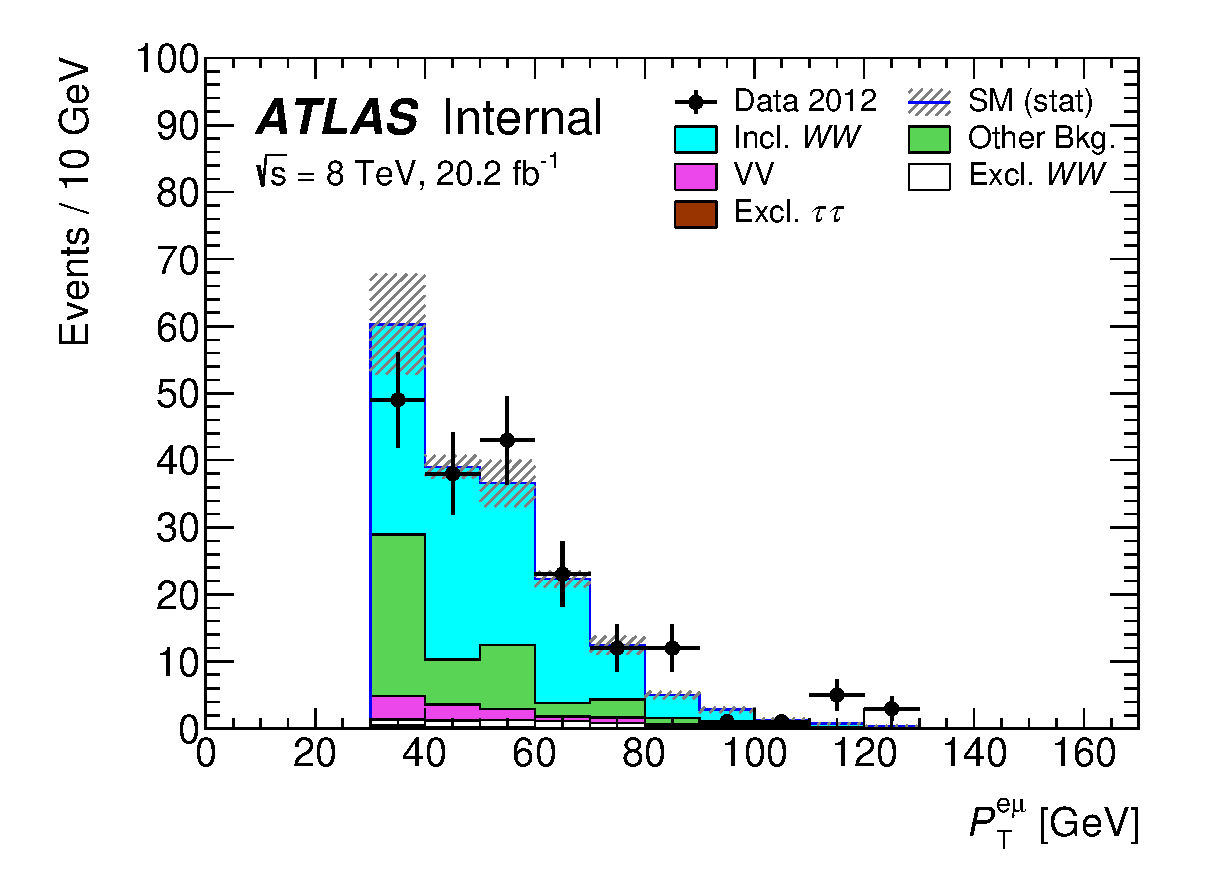
\includegraphics[width=\textwidth]{figures/emme-xtraTracks-Ptll-lin.eps}
\end{subfigure} 
\caption{Plots showing \memu, \dFem, \mT\ and \pTemu\ distributions in the inclusive $\WW$-rich region}
\label{fig:xtrkWWplots}
\end{figure}

\par The true value of the sum of inclusive \WW\ and other backgrounds in this control region     
is bound by two estimates. The upper bound is the observed number of events in data, minus the 
sum of $VV$ and exclusive backgrounds. The lower bound is a special case where there is no 
contribution from the other backgrounds, leading to contribution only from the inclusive \WW, as 
predicted by \PowhegPythiaEight. These two estimates were extrapolated to a region with the same selection criteria but the 
nominal \DZ\ selection.\footnote{In other words, extrapolated from the 1 to 4 track region to the 0 track region}
In this region, the lower bound corresponds to the optimistic case where the other background 
contribution is completely rejected by \DZ, while the upper 
bound corresponds to the case where all observed candidates in the `1 to 4'-track control region are suppressed 
by the same factor as the inclusive $\WW$ process. The average of the two estimates was taken as the 
better estimate to the true value of the sum of inclusive \WW\ and other backgrounds, when the nominal 
\DZ\ selection criterion was applied. Comparing this estimate to the prediction by \PowhegPythiaEight, 
a flat scale factor was extracted to correct for overall exclusivity mis-modelling by Monte Carlo 
simulation. 

\par The extrapolation of upper and lower bounds from the 1 to 4-track region to the nominal \DZ\ region 
was done through 

\begin{equation}
N^{\textrm{Estimated}}_{0} = N^{\textrm{Estimated}}_{1-4} 
                       \times \frac{N_{WW,0}^{\textrm{Predicted}}}{N_{WW,1-4}^{\textrm{Predicted}}}.
\end{equation} 

Here, $N^{\textrm{Estimated}}_{0}$ and $N^{\textrm{Estimated}}_{1-4}$ 
are the estimates for the lower bound or upper bound in the nominal \DZ\ and 1 to 4-track 
region respectively. $N_{WW,0}^{\textrm{Predicted}}$ 
and $N_{WW,1-4}^{\textrm{Predicted}}$ are respectively the number of inclusive $\WW$ events predicted 
by $\PowhegPythiaEight$ for the zero-track and 1 to 4-track regions. 
Extrapolation of the lower bound is trivial: since $N^{\textrm{Estimated}}_{1-4}=N_{WW,1-4}^{\textrm{Predicted}}$ 
the estimate in the nominal \DZ\ region $N^{\textrm{Estimated}}_{0}$ becomes $N_{WW,1-4}^{\textrm{Predicted}}$. 
For upper bound assumes that other backgrounds can be extrapolated using  
$N_{WW,0}^{\textrm{Predicted}}/N_{WW,1-4}^{\textrm{Predicted}}$. The average of 
these two estimates was taken as the overall estimate. Half the difference of the two estimates was taken 
as an additional contribution to the uncertainty in this extrapolation. 

\par This extrapolation yields an estimate of 6.6$\pm$2.5 inclusive \WW\ events in the \DZ\ region. In other 
words, for $\PowhegPythiaEight$ prediction to match this value, a normalization factor of 0.79 was necessary. 
So in the signal region, a 0.79 scale factor was applied to the inclusive \WW\ prediction from Monte Carlo 
simulation. 
 


\section{Validation of background modelling}
\label{sec:exclHCR}
\par The section discusses validation of background modelling. Two regions in data were 
defined to validate modelling of exclusive and inclusive backgrounds. 

\par Since the major 
exclusive background is exclusive \WW, a region that enhanced such events is discussed here. 
This region also contains a significant contribution from inclusive \WW, so it demonstrates the 
validity of the inclusive \WW\ modelling techniques discussed in the preceding sections. 

\par Although \Ztau\ events were not expected to be very significant in the signal region, 
studying background composition in a region of data rich in \Ztau\ events reinforced that 
all the other backgrounds were reasonably well-modelled. 

\subsection{Exclusive \WW}
\label{sec:exclWWCR}
\par While the 1 to 4-track region introduced in Table~\ref{tab:incWWCR} was 
rich in inclusive \WW\ events, replacing the 1 to 4-track selection criterion with the 
nominal \DZ\ selection criterion suppressed the inclusive \WW\ events and enhanced 
the exclusive \WW\ events. This is the exclusive \WW\ validation region. 

\par Although this region was discussed in Section~\ref{sec:incWW}, validation kinematic 
distributions are presented in this section. Figure~\ref{fig:exclWWCR} shows such 
distributions. The inclusive \WW contribution was scaled by 0.79 as discussed in Section~\ref{sec:incWW}. 
The exclusive \WW\ and $\tau\tau$ estimates were scaled by \fgam. Contributions from 
$VV$ were very small. Any other background processes were insignificantly small in comparison to 
the inclusive \WW\ contribution. 
  
\begin{figure}[!h]
\begin{subfigure}{0.5\textwidth}
   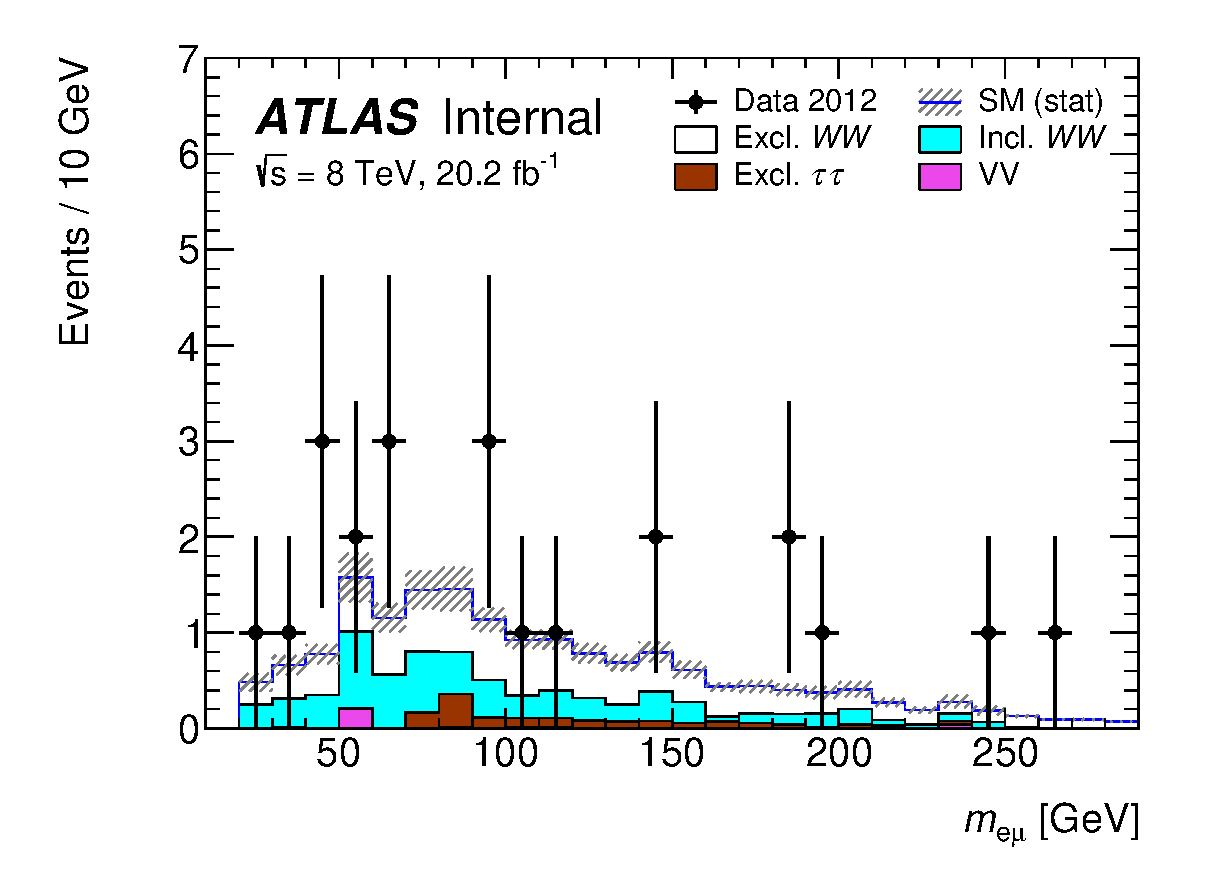
\includegraphics[width=\textwidth]{figures/emme-CutExcl1mm-Mll-lin.eps}
\end{subfigure}
\begin{subfigure}{0.5\textwidth}
   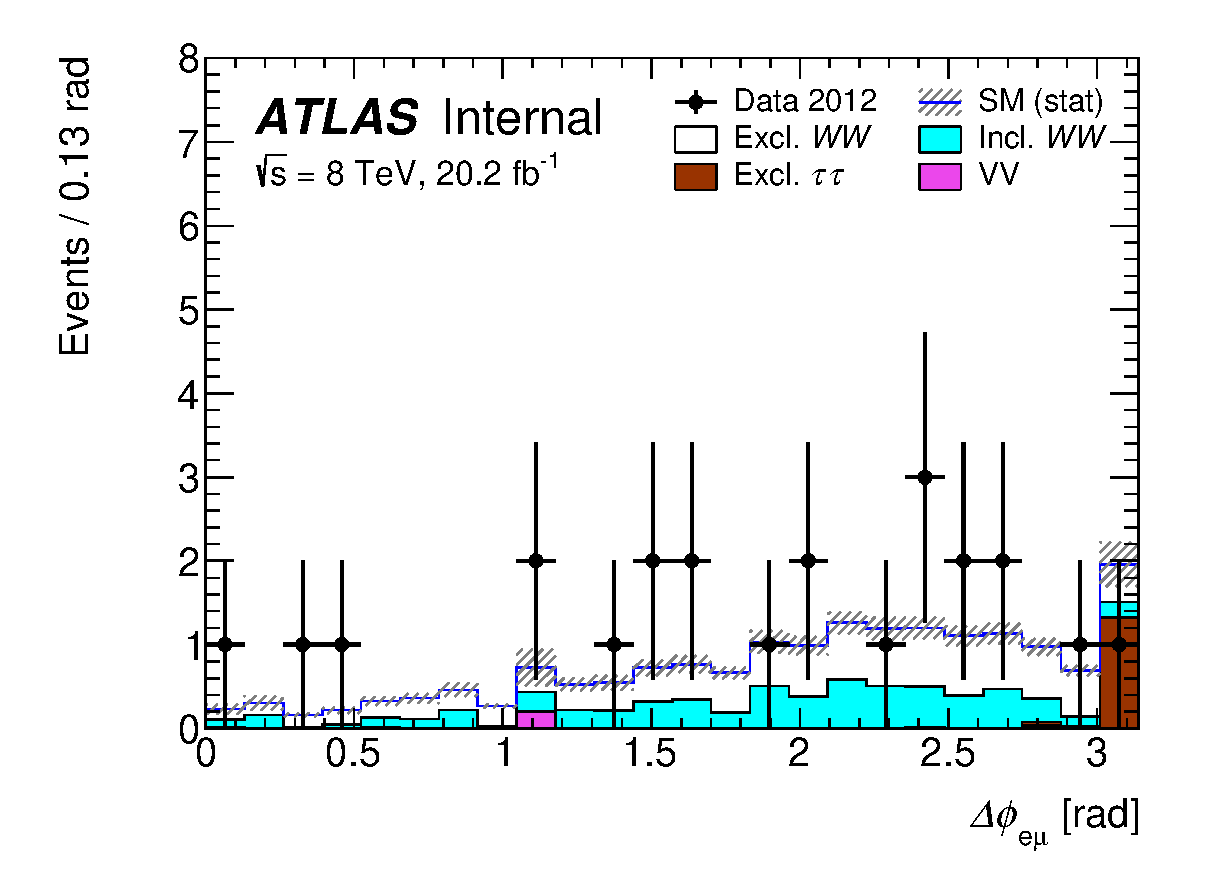
\includegraphics[width=\textwidth]{figures/emme-CutExcl1mm-DPhill-lin.eps}
\end{subfigure} 
\begin{subfigure}{0.5\textwidth}
   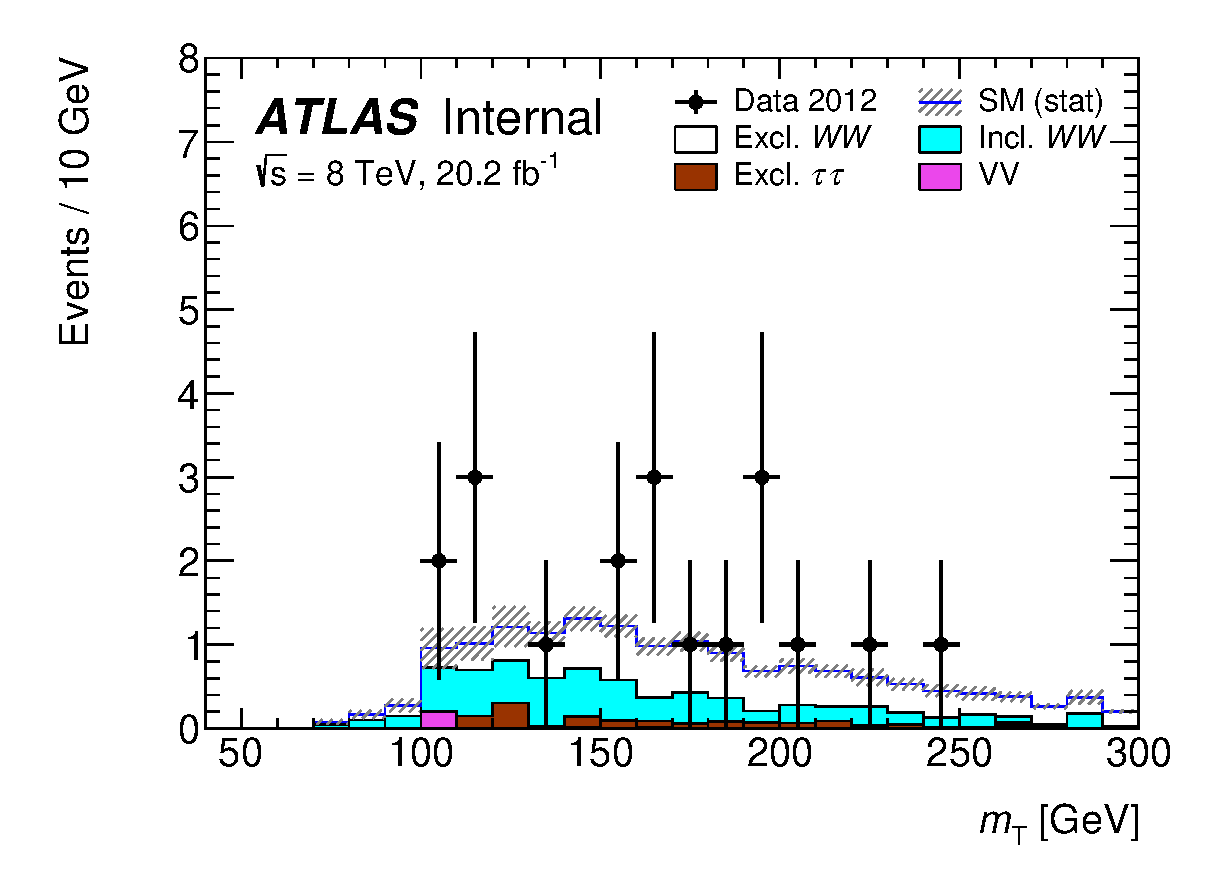
\includegraphics[width=\textwidth]{figures/emme-CutExcl1mm-MT-lin.eps}
\end{subfigure} 
\begin{subfigure}{0.5\textwidth}
   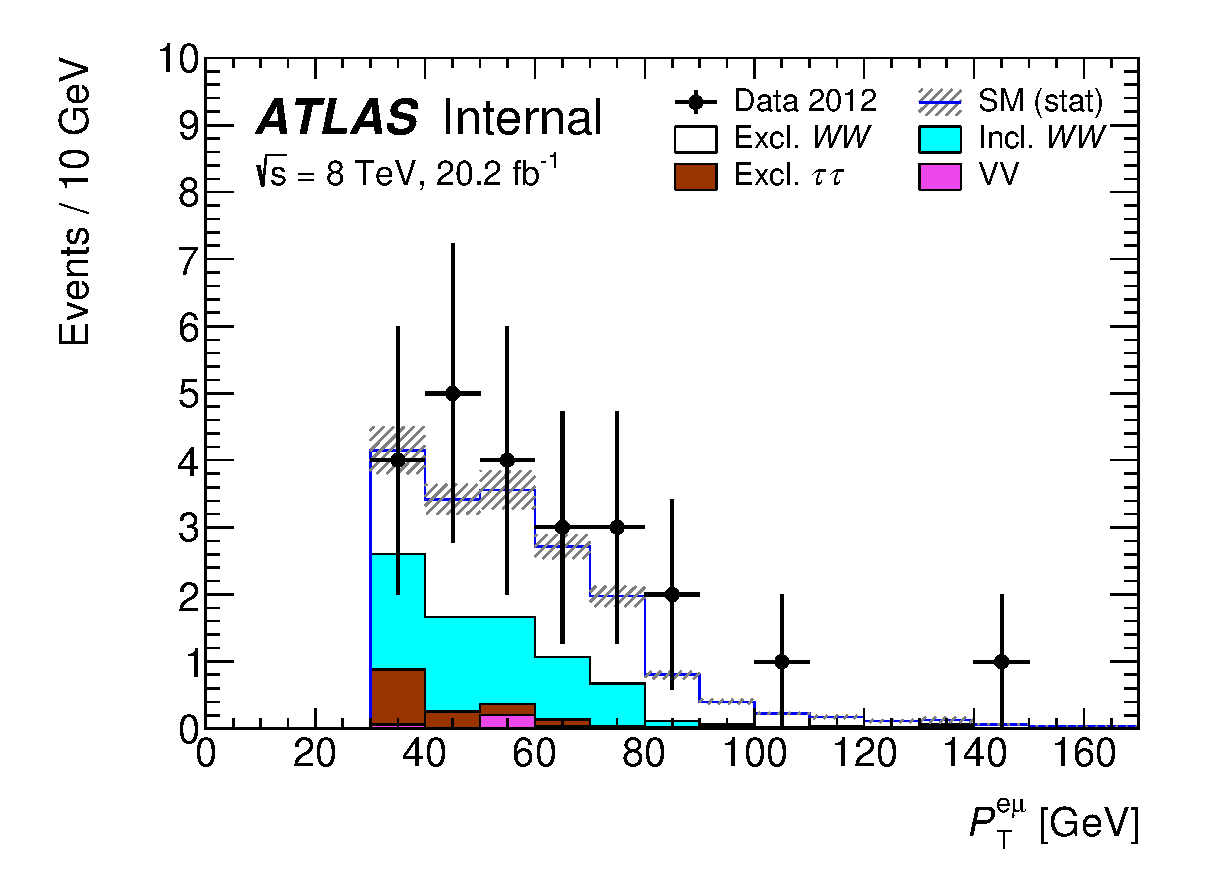
\includegraphics[width=\textwidth]{figures/emme-CutExcl1mm-Ptll-lin.eps}
\end{subfigure} 
\caption{Plots showing \memu, \dFem, \mT\ and \pTemu\ distributions in the exclusive \WW\ validation region}
\label{fig:exclWWCR}
\end{figure}

\par Overall Figure~\ref{fig:exclWWCR} shows reasonable agreement between data and 
predictions. A slight underestimation of exclusive \WW\ was observed across all the 
distributions. From counting the yields from all the processes and comparing them 
with the observed data, a normalization factor of 1.57$\pm$0.62 was extracted, to 
be additionally applied to the exclusive \WW\ contributions in the signal region. 
The uncertainty in this normalization factor resulted from propagation of 
uncertainties of each of the numbers that went into the calculation. 

\subsection{Inclusive \Ztau}
\label{subsec:ztau}
\par A \Ztau+jets-rich region was defined in data  
to validate background modelling in an environment dominated by inclusive processes. 
Table~\ref{tab:ZtauCR} summarizes the definition of this region.
Figure~\ref{fig:ZtauCR} shows some kinematic distributions in this validation 
region, after all the selection criteria summarized in Table~\ref{tab:ZtauCR} were applied.
The general slight disagreement between data and simulation was  
attributed to the mismodelling of the transverse momentum of the \Zboson, $p_T^Z$.
This mismodelling is well documented in Ref~\cite{Chelstowska:1636127}. While considerable efforts 
are normally applied to reweight the \Zboson\ \pt, \Ztau\ events were not 
a primary background in this analysis so such reweighting was observed to have insignificant effects on results. 

\begin{table}[!h]
\centering
\begin{tabular}{|l|r|}
\hline
& 	Selection 															\\
\hline\hline
 \multirow{3}{*}{Preselection }									&		Lepton $p_{\mathrm{T}}$ 25, 15 GeV	 		\\
																					&		OS and different flavour leptons 												 			\\
																					&		$m_{\ell\ell} > 10$ GeV 								\\
\hline
 \multirow{2}{*}{\Ztau}								&		$p_{\mathrm{T}}^{\ell\ell}<$30 GeV 				\\
									& 	$m_{\ell\ell}<80$ GeV 							\\
\hline
 \multirow{2}{*}{Exclusivity}	 					&		$|z_0^1-z_0^2|<1.0$ mm 							\\
											& 	$\Delta z_0 > 1.0$ mm 				\\	
\hline
\end{tabular}
\caption{\Ztau\ validation region definition.}
\label{tab:ZtauCR}
\end{table}

\begin{figure}[!h]
\begin{subfigure}{0.5\textwidth}
   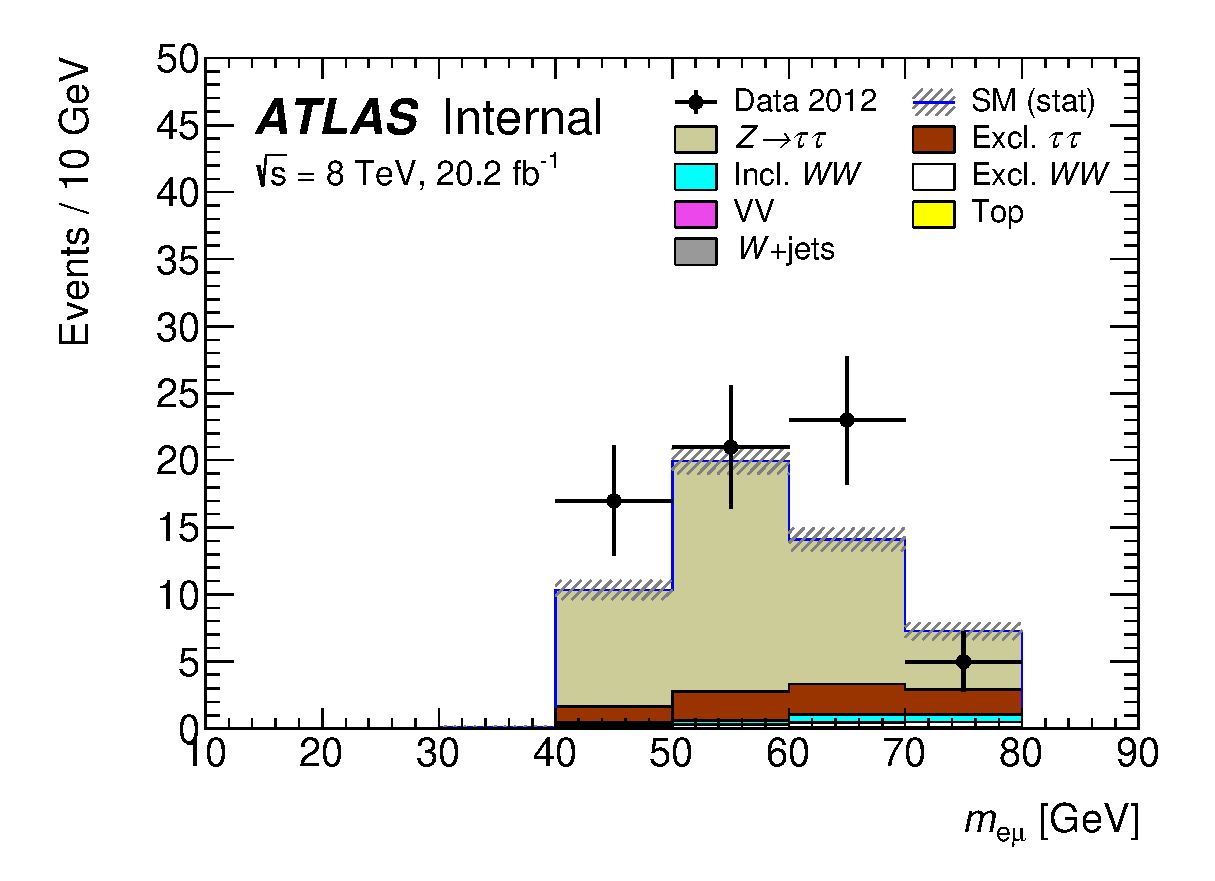
\includegraphics[width=\textwidth]{figures/emme-CutTopoMll-Mll_ztau-lin.eps}
\end{subfigure}
\begin{subfigure}{0.5\textwidth}
   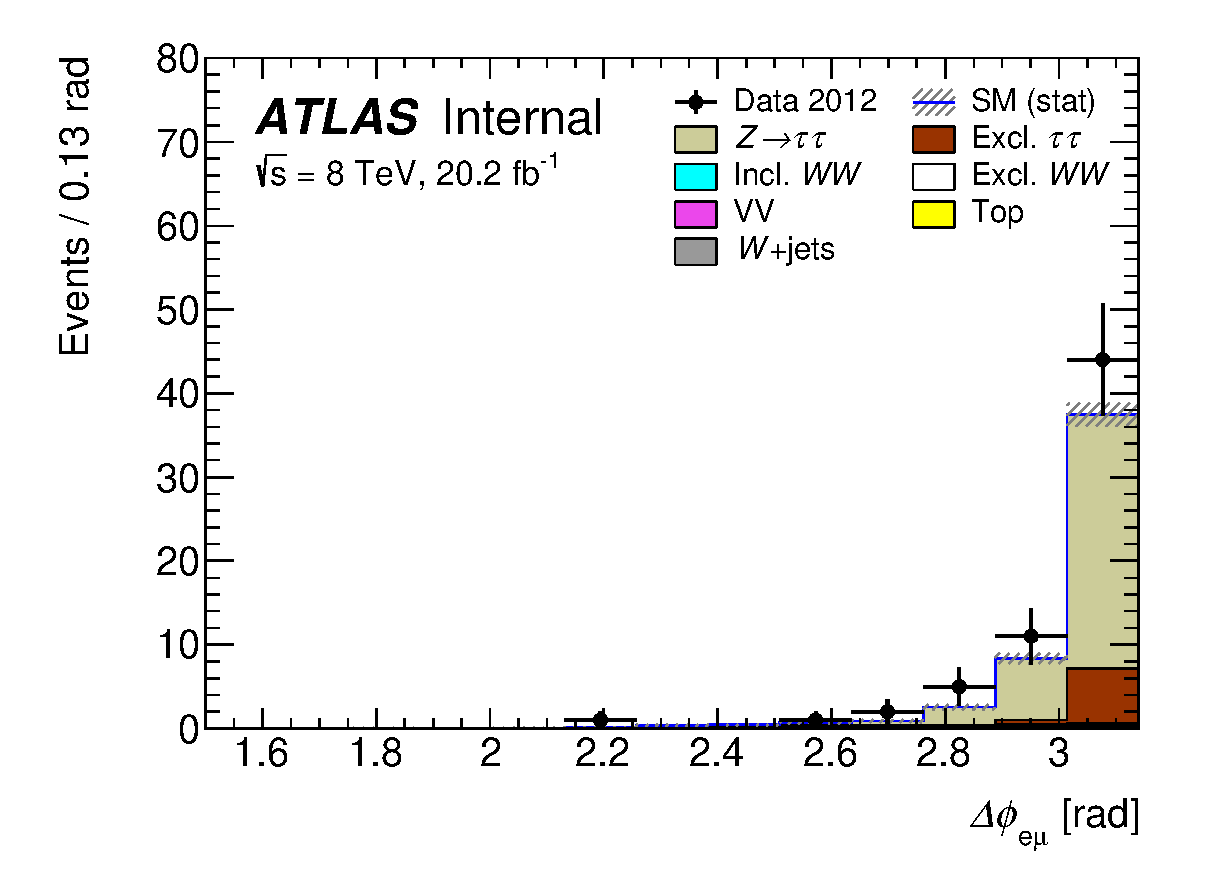
\includegraphics[width=\textwidth]{figures/emme-CutTopoMll-DPhill_ztau-lin.eps}
\end{subfigure} 
\begin{subfigure}{0.5\textwidth}
   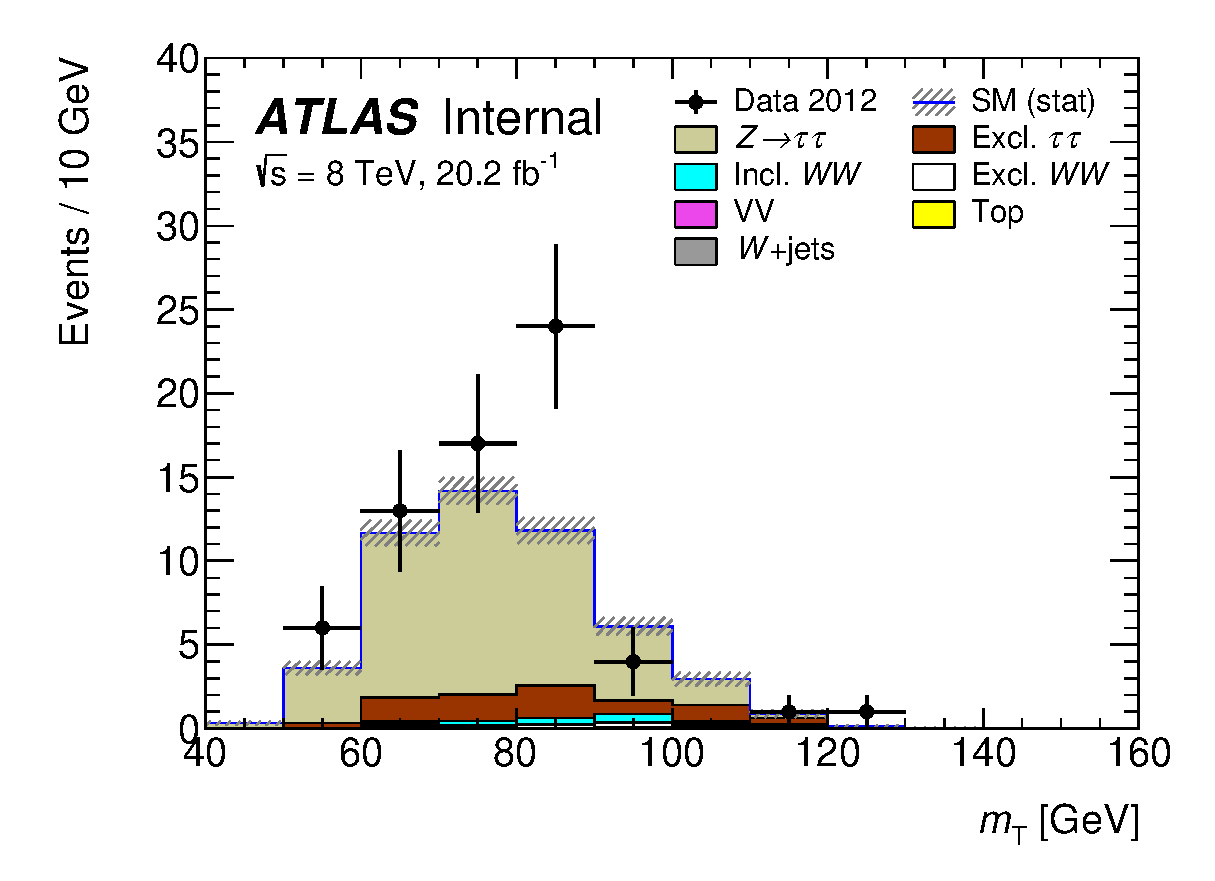
\includegraphics[width=\textwidth]{figures/emme-CutTopoMll-MT_ztau-lin.eps}
\end{subfigure} 
\begin{subfigure}{0.5\textwidth}
   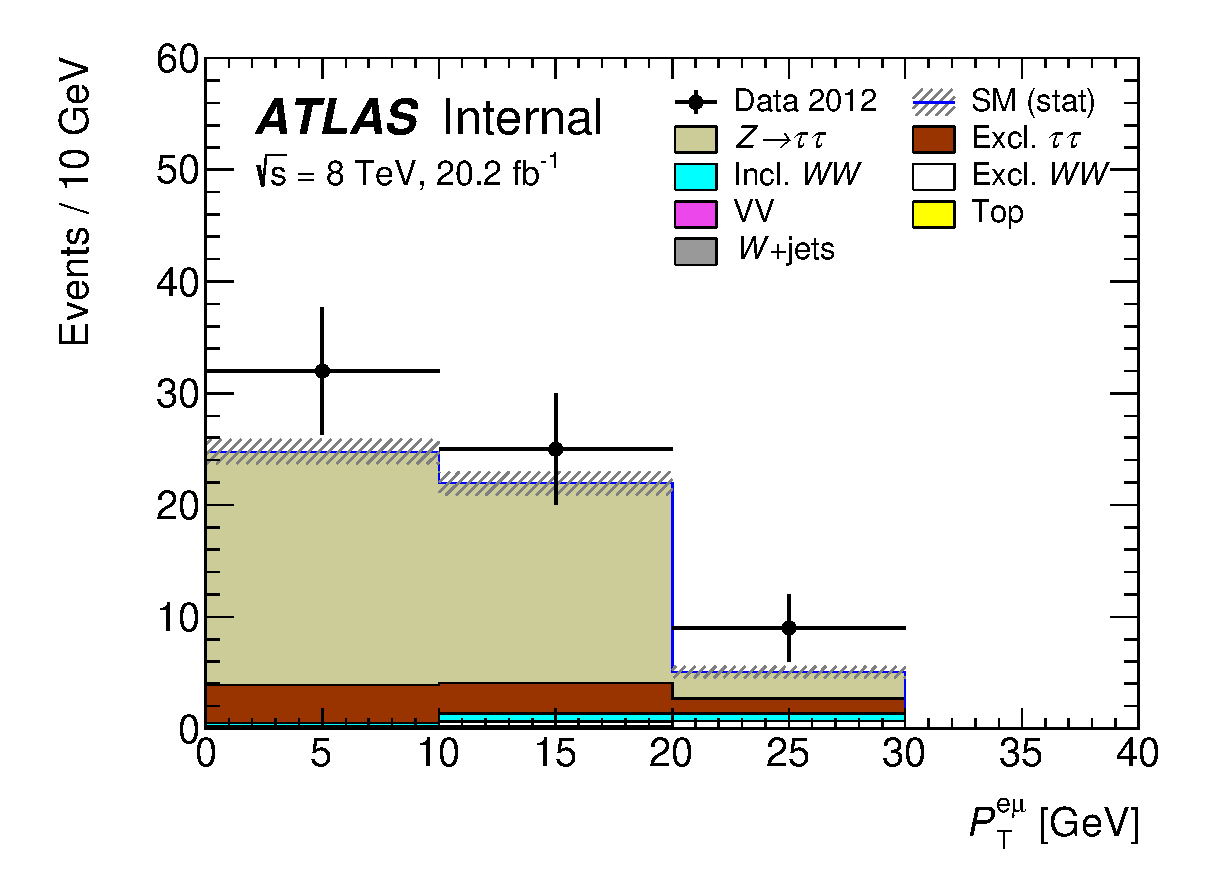
\includegraphics[width=\textwidth]{figures/emme-CutTopoMll-Ptll_ztau-lin.eps}
\end{subfigure} 
\caption{Plots showing \memu, \dFem, \mT\ and \pTemu\ distributions in the \Ztau\ validation region}
\label{fig:ZtauCR}
\end{figure}


\section{Systematic Uncertainties and Statistical analysis}
\label{sec:exclHUnc}
\par This section summarizes the sources of systematic uncertainties in this search. 
The most important of these sources are listed in table~\ref{tab:mainSystematics}.
The errors on the various scale factors, $f_{\gamma} = 3.30 \pm 0.23$
and $f_{EL} = 0.76 \pm 0.04 \pm 0.07$  
were included in the analysis as systematic uncertainties. 
For $Z$+jets, the estimate of 20\% comes from the exclusivity  
calibration method described in Section~\ref{sec:exclCalib}. Details on the 
flux factor and $WW$ background uncertainties are discussed in Sections~\ref{sec:flux} and {sec:incWW}
respectively. 

\begin{table}[!h]
 \centering
 \resizebox{\textwidth}{!}{
   \begin{tabular}{|l|ccccc|}
\hline
 Source of Uncertainty     & Exclusive $WW$  & Exclusive Higgs & Exclusive $\tau\tau$ &  Inclusive $WW$ & $Z$+jets\\
     \hline\hline
     Exclusivity              & 10\% & 10\% & -- & -- & -- \\
     $f_{\gamma}$           & 7\% & -- & -- & -- & -- \\
     $f_{EL}$            & -- & -- & 10\% & -- & -- \\
     Background        & -- & -- & -- & 38\% & 20\% \\
     \hline
   \end{tabular}
 }
 \caption{Most important sources of systematic uncertainties and their contribution
          to the event yields. The largest ones come from estimates of background. 
          Dashed lines imply that the source was not directly applicable to 
          that particular process.}
 \label{tab:mainSystematics}
\end{table}

\par The systematic uncertainties associated to the physics objects were estimated using 
using methods discussed in Chapter~\ref{obj}. They are listed in table~\ref{tab:systs}. 
 The systematics in tables 
\ref{tab:mainSystematics} and \ref{tab:systs} are uncorrelated, so they 
were added in quadrature.

\begin{table}
\centering
        \resizebox{0.95\textwidth}{!}{
\begin{tabular}{|lllll|rrrr|}
\hline
 													&	&	&	&	 Source of Uncertainty																& Excl. Higgs [\%]		 & Incl. WW	[\%]	 & Excl. WW	[\%]	 & ggF H. [\%]		\\ 
 \hline\hline 
													& & & &  Electron Resolution						& 0.02  	  & 0.05  	  & 0.06  	  & 0.05  	 \\

													& & & &  Electron Energy Scale					& 0.75  	  & 0.24  	  & 0.59  	  & 0.67  	 \\

													& & & &  Muon Energy Scale							& 0.11  	  & 0.03  	  & 0.04  	  & 0.07  	 \\

													& & & &  Electron ID \& Reco.						& 1.55  	  & 1.26  	  & 1.28  	  & 1.35  	 \\

													& & & &  Muon ID												& 0.32  	  & 0.32  	  & 0.32  	  & 0.32  	  \\ 

													& & & &  Single Electron Trigger SF			& 0.45  	  & 0.31  	  & 0.32  	  & 0.35  	 \\

													& & & &  Single Muon Trigger SF					& 0.64  	  & 0.47  	  & 0.53  	  & 0.53  	 \\

													& & & &  Elec-Muon Trigger SF						& 0.01  	  & 0.01  	  & 0.01  	  & 0.01  	 \\
\hline
													& & & & \textbf{Total Lepton}                     & \textbf{1.92}      & \textbf{1.44}			& \textbf{1.57}      & \textbf{1.67}     \\ 
\hline
 \ldelim\{{10}{2mm}[JES]	 	& & & &	 EtaModelling						& --  	  & 0.33  	  & --  	  & --  	 \\

                          	& & & &  EtaStatMethod					& --  	  & 0.08  	  & --  	  & --  	 \\

														& & & &  FlavComp								& --  	  & 0.04  	  & --  	  & --  	 \\

														& & & &  FlavResp								& --  	  & 0.45  	  & --  	  & --  	 \\

														& & & &  HighPt									& --  	  & 0.04  	  & --  	  & --  	 \\

														& & & &  NPDetector1						& --  	  & 0.17  	  & --  	  & --  	  \\ 

														& & & &  NPModelling1						& --  	  & 0.45  	  & --  	  & --  	 \\

														& & & &  NPV										& --  	  & 0.16  	  & --  	  & --  	 \\

														& & & &  PilePt									& --  	  & 0.04  	  & --  	  & --  	 \\

                          	& & & &  PileRho								& --  	  & 0.26  	  & --  	  & --  	 \\
\hline
														& & & &  \textbf{Total JES}              & \textbf{--}			& \textbf{0.8}      & \textbf{--}      & \textbf{--}     \\ 
\hline											& & & & Luminosity							& 1.90      & 1.90      & 1.90      & 1.90      \\
\hline
\end{tabular}
}
\caption{List of all systematic uncertainties associated with the reconstruction of physics objects. Chapter~\ref{obj} 
discusses methods with which these uncertainties were calculated. The individual uncertainties were assumed to be 
uncorrelated so they were added in quadrature.}
\label{tab:systs}
\end{table}

\par The statistical framework used to evaluate results of this search are identical to those used in the 
search for the charged Higgs boson. See Section~\ref{sec:systsCh} for more details.  


\section{Results}
\label{sec:exclHres}
\subsection{Expected and observed event yields}
\par After the event selection criteria for the signal region was finalized, and the background 
modelling validated, final kinematic distributions in the signal region were examined. 
Figure~\ref{fig:exclHsr} shows n-1 distributions for \dFem, \memu, \mT\ and \pTemu. 
N-1 distributions show event yields and shapes in the signal region, minus the 
selection criteria specific to the distribution being plotted. All the scale factors 
discussed in the preceding sections were applied to correctly model the backgrounds. 
For the exclusive \WW\ process, \fgam\ was multiplied by 1.57 to match validation 
results observed in Section~\ref{sec:exclHCR}. The inclusive \WW\ process was scaled 
by 0.79. As discussed in Section~\ref{sec:incWW}, applying this background implicitly 
adds the \Ztau\ background to the inclusive \WW\ background. The rest of the backgrounds 
were scaled by their respective scale factors to account for the mis-modelling of the 
underlying event in simulation.

\par A summary of the yields in the signal region is shown in Table~\ref{tab:Higgsyields}.    
Six events were observed in data, while 3.00$\pm$0.78 events were expected from all 
the background processes; 0.023$\pm$0.003 events were expected from signal, where the 
quoted uncertainty is the sum in quadrature of systematic uncertainties and simulation 
statistical uncertainties. 

\begin{table}[!h]
\centering
        \resizebox{\textwidth}{!}{
\providecommand{\cutflowTitle}{}
\begin{tabular}{|l|rrr|rrr|}
\hline
 																							& Excl. $H$ Signal				& Data 		& Total Bkg 		& Incl. $\WW$ 	& Excl. $W^{+}W^{-}$ & Other Bkg 								 \\
\hline\hline
Preselection 																	& 0.065 $\pm$ 0.005 			& 129018 	& 120090				& 12844 				& 43  								& 107200\\
 $\pTemu>$30~\GeV, $\memu<55$~\GeV, $\dFem<1.8$ & 0.043 $\pm$ 0.004 			& 18568 	& 17060  				& 2026 					& 5.7									& 15030 \\
\DZ\ requirement 															& 0.023 $\pm$ 0.003 			& 8 			& 4.7 $\pm$ 1.3 & 1.4 $\pm$ 0.5 & 3.1 $\pm$ 1.3       & 0.2 $\pm$ 0.1  \\
$\mT<140$~\GeV [Signal Region] 							& 0.023 $\pm$ 0.003  			& 6 			& 3.0 $\pm$ 0.8 & 1.0 $\pm$ 0.4 & 1.8 $\pm$ 0.8       & 0.2 $\pm$ 0.1  \\
\hline
\end{tabular}
}
\caption{Summary of signal and background yields at different stages
  of the Higgs boson event selection. Only major background sources are listed explicitly. All 
the other background sources are summed up in the `Other'
category. For the background, the uncertainties are only shown for the yields after exclusivity selection, where they are 
relevant for the measurement. They include the systematic and
statistical components, added in quadrature.}
\label{tab:Higgsyields}
\end{table}

\begin{figure}[!h]
\begin{subfigure}{0.5\textwidth}
   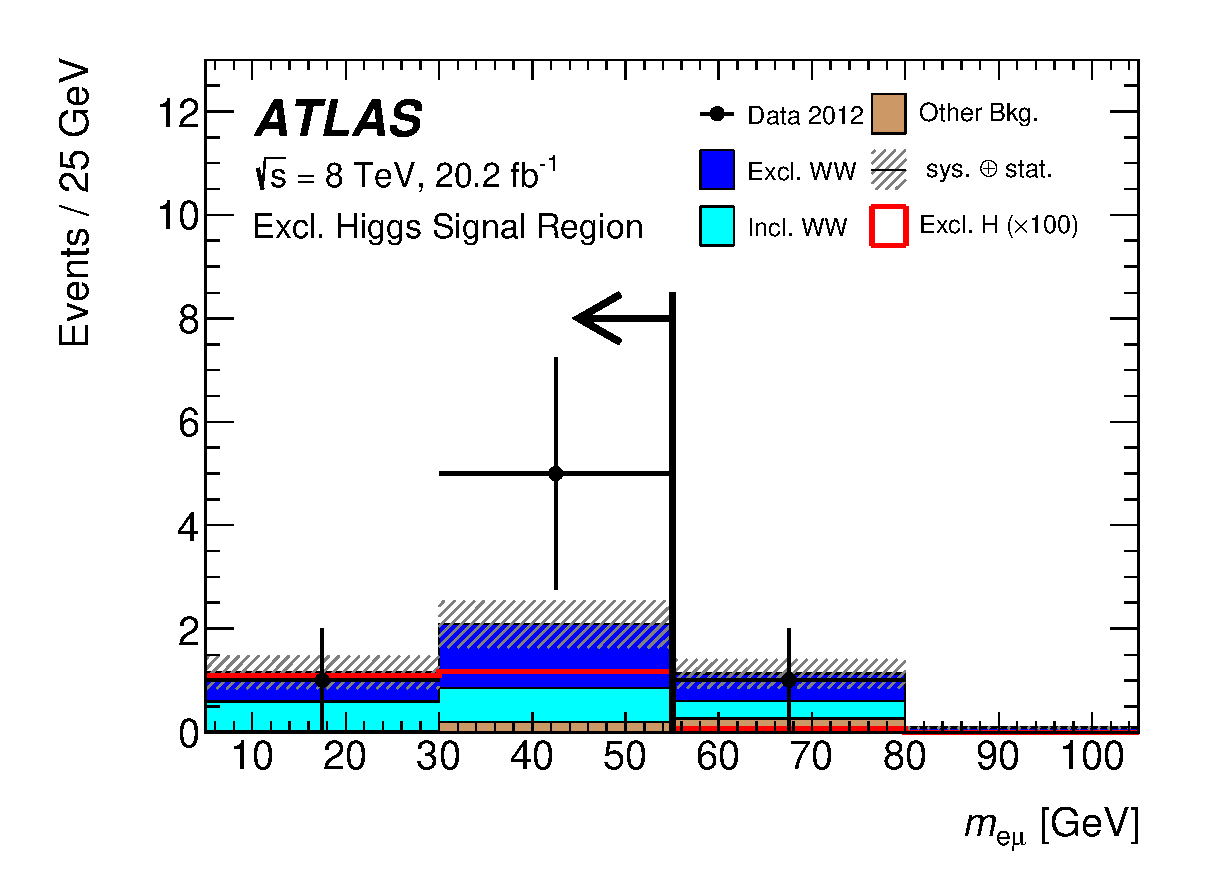
\includegraphics[width=\textwidth]{figures/emme_CutSR_Mll_nMinus1_MllnMinusOne.eps}
\end{subfigure}
\begin{subfigure}{0.5\textwidth}
   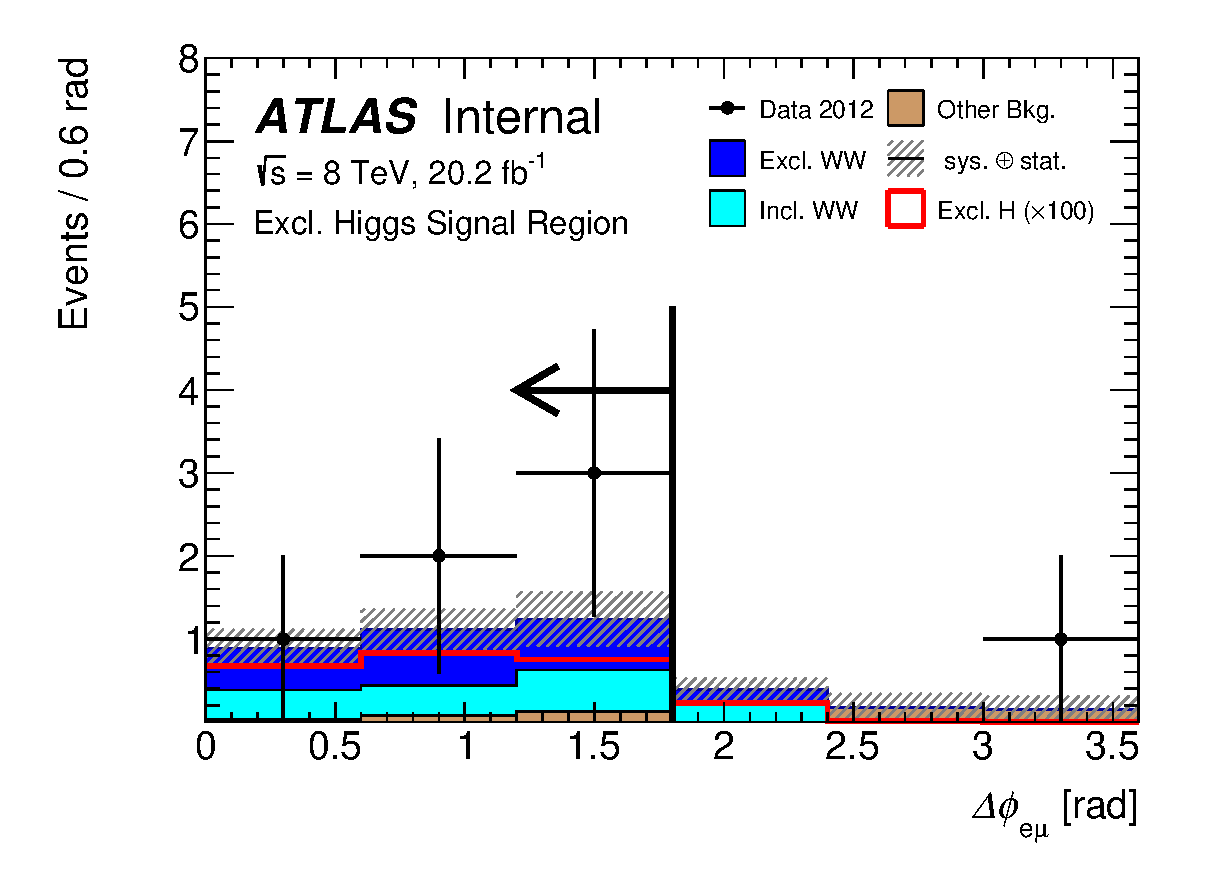
\includegraphics[width=\textwidth]{figures/emme_CutSR_DPhill_nMinus1_DPhillnMinusOne.eps}
\end{subfigure} 
\begin{subfigure}{0.5\textwidth}
   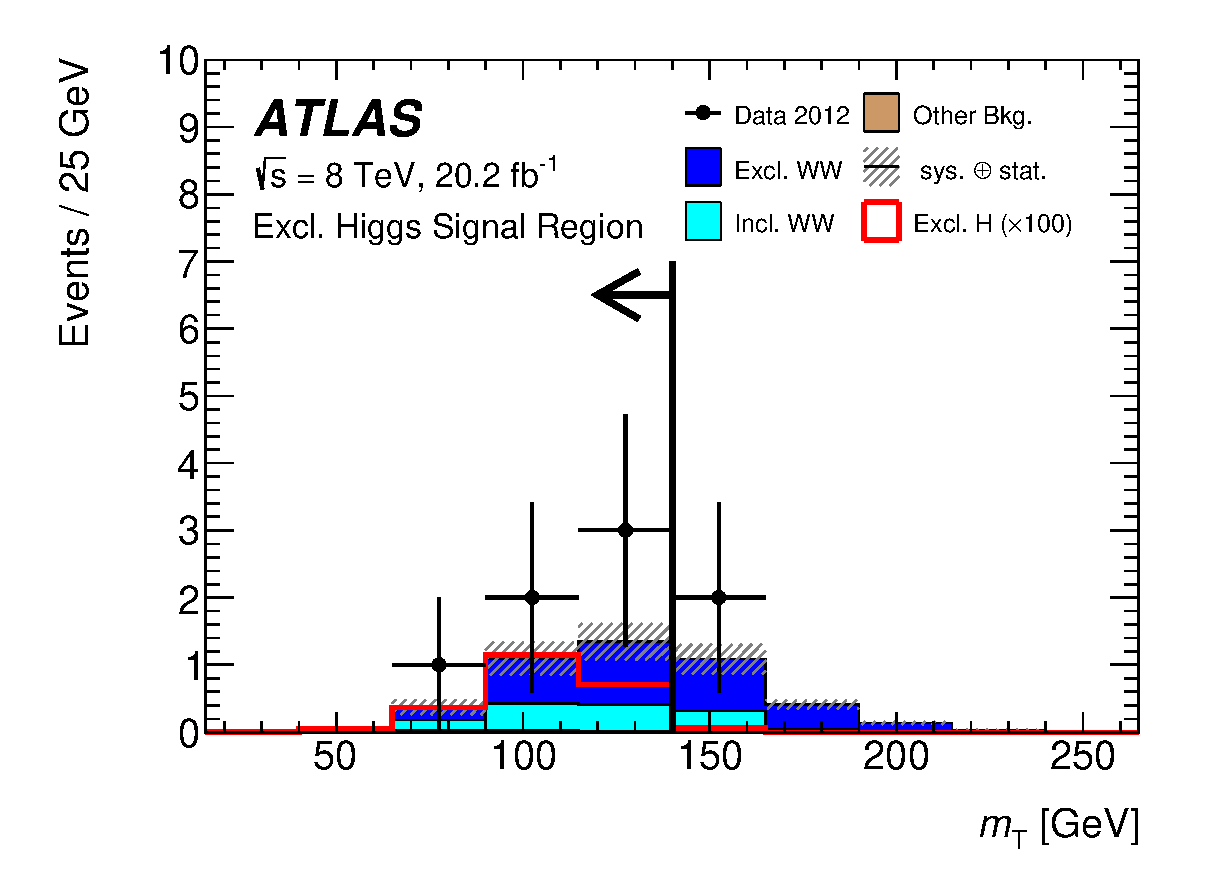
\includegraphics[width=\textwidth]{figures/emme_CutSR_MT_nMinus1_MTexcl.eps}
\end{subfigure} 
\begin{subfigure}{0.5\textwidth}
   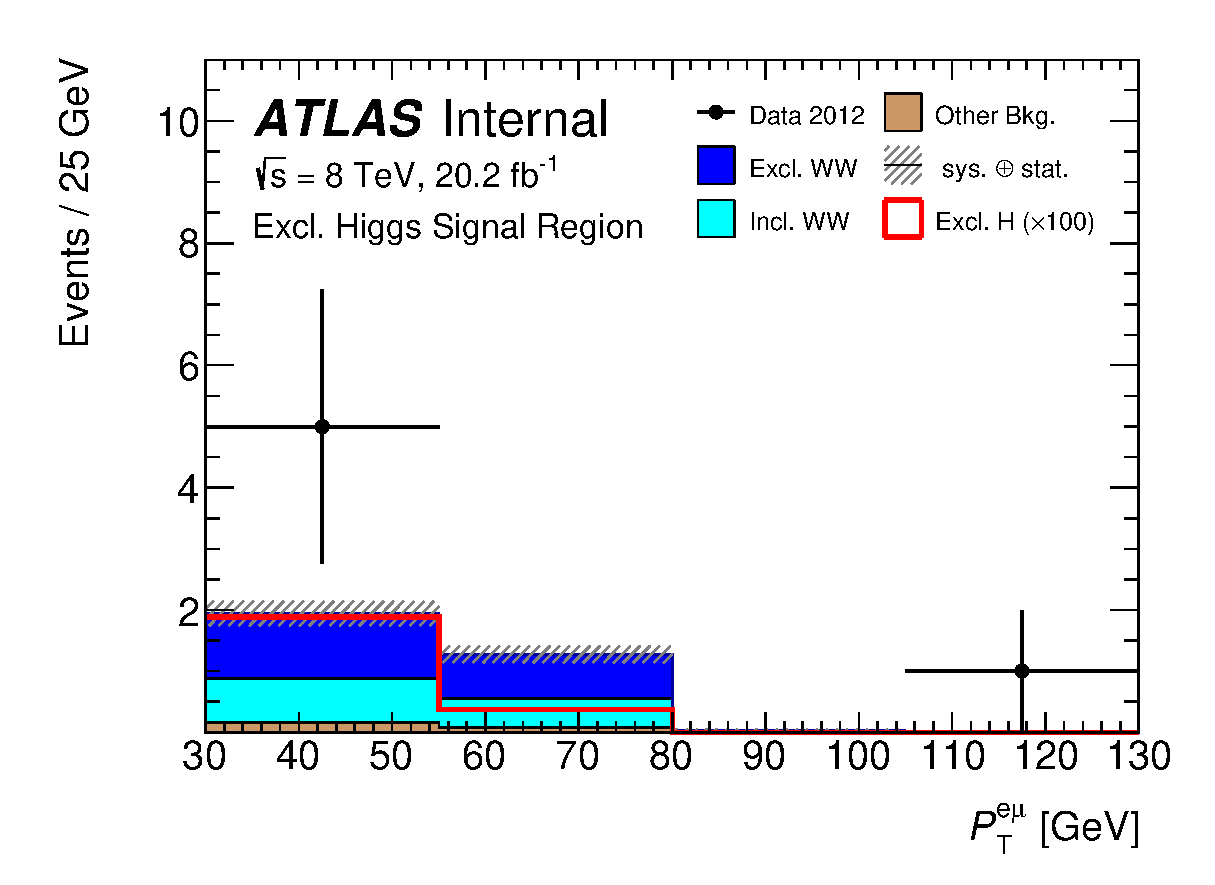
\includegraphics[width=\textwidth]{figures/emme_CutSR_Ptll_nMinus1_PtllnMinusOne_130.eps}
\end{subfigure} 
\caption{Plots showing \memu, \dFem, \mT\ and \pTemu\ distributions in the signal region, minus the selection criteria for the variable 
being plotted}
\label{fig:exclHsr}
\end{figure}


\subsection{Statistical Analysis}
\par The results presented in the preceding sub-section were tested for evidence of exclusive Higgs 
production in LHC Run I data. For a Standard Model Higgs boson with $m_{\text{H}} = 125~\GeV$, 
$\sigma^{Exp}_{H}$ was set at 
1 to make the parameter of interest $\mu=\sigma^{Obs}_{H}$. The test statistic $q_0$, where $\mu=0$ 
in Equation~\ref{eq:testStat}, was used to test the compatibility 
of observed data with the background-only hypothesis. The rest of the statistical analysis is identical 
to that described in Section~\ref{sec:chStat}, including the treatment of systematic uncertainties.
The discrepancy between the observed data and expected event yields corresponded to a 1.1$\sigma$ 
upward fluctuation from the expected Standard Model results. This fluctuation is not significant enough 
to prove existence of the exclusive Higgs boson. Expected limits on the exclusive Higgs boson 
cross section were therefore set, using the $CL_s$ procedure, where $CL_s(\mu)$ is defined as in Equation~\ref{eq:cls}. 

\par Table~\ref{tab:models} shows a summary of the 95\% CL upper limits on the exclusive 
Higgs boson total production cross-section.
The observed upper limit is 1.2 pb, which is 1.1$\sigma$ higher than the expected 
upper limit of 0.7 pb. The statistical uncertainty in the predicted background dominates the
uncertainty involved in calculating this upper limit, 
while systematic uncertainties worsen the upper limits by at most 10\%.
This upper limit value is 400 times the cross-section predicted~\cite{Khoze}.
However, the limit would not change if the model prediction, which is for
elastic production only, increased by an order of magnitude. This limit calculation 
inherently assumes that the acceptance and efficiency for dissociative
events is not significantly different than for elastic events, hence
the associated systematic uncertainty is insignificant.

\begin{table}
\centering
%\resizebox{0.5\textwidth}{!}{
\begin{tabular}{|cc|c|cc||r|}
\hline
$+2\sigma$ [pb] & $+1\sigma$ [pb] & Expected [pb] & $-1\sigma$ [pb] & $-2\sigma$ [pb] & Observed [pb] \\
\hline\hline
 1.6 & 1.0  & 0.7 &  0.5 &  0.4 & 1.2 \\
\hline 
\end{tabular}
%}
\caption{Upper limits on $\sigma_H$ [pb] at 95\% CL. The $\pm 1\sigma$ and $\pm 2\sigma$ uncertainties quoted here are on the expected upper limit.}
\label{tab:models}
\end{table}



%
%\begin{chapsummary}
%\par A search for evidence of the exclusive Higgs boson in LHC's Run I data-set was performed, 
%in the channel where the Higgs boson decays to a pair of \Wpm\ which subsequently decay 
%leptonically. Decay of \Wpm\ to $\tau$ leptons were allowed only if the $\tau$ lepton 
%decayed leptonically. A new method for separating exclusive events from inclusive events was devised, specifically for 
%isolating exclusive Higgs events. This method was tested in both simulation and data, correcting any mis-modelling 
%observed in simulation. Overall, background treatment was validated in two regions of data and observed to 
%be reasonable. In the signal region, six events were observed in data while 3.00$\pm$0.78 events were expected from all 
%the background processes. This discrepancy was evaluated to be 1.1$\sigma$ higher than expected, and hence 
%not high enough to conclude the presence of exclusive Higgs events in the data-set. Upper limits were therefore 
%set on the total production cross section of the exclusive Higgs boson. The set limits were 400 times 
%the cross section predicted by the most popular model for the production of the exclusive Higgs boson.  
%\end{chapsummary}
